\documentclass[12pt, a4paper]{article}

\usepackage[left=3cm,top=3cm,right=2cm,bottom=2cm]{geometry}
\usepackage[brazilian]{babel}
\usepackage{amsfonts, amsmath, amssymb}
\usepackage{graphicx, float, caption, subcaption}
\usepackage[hidelinks]{hyperref}
\usepackage{booktabs}

\title{(Universidade de São Paulo)\\
Discretizações de Diferenças Finitas para a Equação de Advecção-Difusão: Análise de Estabilidade e Efeitos do Número de Péclet}

\author{
Métodos Numéricos em Equações Diferenciais\\
Docente: Fabrício Simeoni de Sousa\\[.2cm]
\begin{tabular}{c@{\qquad}c}
Kainã Alves Tureso & Vinícius de Sá Ferreira\\
15466391           & 15491650\\
\end{tabular}
}

\date{\today}
\graphicspath{{../graphs}}

\renewcommand{\arraystretch}{1.3}
\newcommand{\bb}[1]{\mathbb{#1}}
\renewcommand{\bf}[1]{\mathbf{#1}}
\newcommand{\D}[1]{\Delta#1}
\renewcommand{\O}[1]{\mathcal{O} (#1)}
\newcommand{\Pe}{\bb{P}e}

\begin{document}

    \maketitle

    \tableofcontents

    \section{Formulação do Problema}

    Considera-se a equação diferencial parcial de advecção-difusão
    \begin{equation}
        u_t(x,t) + u_x(x,t) = \frac{1}{\bb{P}e} u_{xx}(x,t), \quad (x,t) \in [0,15] \times [0,12],
    \end{equation}
    onde $\bb{P}e$ denota o número de Péclet, que caracteriza a razão entre os efeitos advectivos e difusivos. Introduz-se a malha uniforme $x_j = j\D{x}$ e $t_n = n\D{t}$, com $j = 0,1,\ldots,N_x$ e $n = 0,1,\ldots,N_t$, e denota-se por $U_j^n$ a aproximação numérica de $u(x_j,t_n)$.

    \section{Discretizações}

    \subsection{Diferenças progressivas no tempo e centradas no espaço}

    Aproximando a derivada temporal por diferenças progressivas de primeira ordem e as derivadas espaciais por diferenças centradas de segunda ordem, obtém-se
    \begin{equation}
        \begin{split}
            &\frac{u(x_j,t_{n+1})-u(x_j,t_n)}{\D{t}} + \O{\D{t}} + \frac{u(x_{j+1},t_n)-u(x_{j-1},t_n)}{2\D{x}} + \O{\D{x}^2}
            \\&= \frac{1}{\bb{P}e} \frac{u(x_{j+1},t_n)-2u(x_j,t_n)+u(x_{j-1},t_n)}{\D{x}^2} + \O{\D{x}^2},
        \end{split}
    \end{equation}
    resultando no esquema numérico
    \begin{equation}
        \frac{U_j^{n+1}-U_j^n}{\D{t}} + \frac{U_{j+1}^n-U_{j-1}^n}{2\D{x}} = \frac{1}{\bb{P}e} \frac{U_{j-1}^n-2U_j^n+U_{j+1}^n}{\D{x}^2},
    \end{equation}
    que pode ser reescrito de forma equivalente como
    \begin{equation}
        \begin{split}
            U_j^{n+1} &= \left(\frac{\D{t}}{\bb{P}e\D{x^2}}+\frac{\D{t}}{2\D{x}}\right)U_{j-1}^n + \left(1-\frac{2\D{t}}{\bb{P}e\D{x^2}}\right)U_j^n + \left(\frac{\D{t}}{\bb{P}e\D{x^2}}-\frac{\D{t}}{2\D{x}}\right)U_{j+1}^n\\[.2cm]
            &= (\alpha+\beta)U_{j-1}^n + (1-2\alpha)U_j^n + (\alpha-\beta)U_{j+1}^n,
        \end{split} \label{eq:centradas}
    \end{equation}
    onde $\alpha = \dfrac{\D{t}}{\bb{P}e\D{x^2}}$ e $\beta = \dfrac{\D{t}}{2\D{x}}$.

    \vspace{.4cm}

    Sob condições de contorno periódicas, define-se $U_{N_x+1}^n = U_0^n$, de modo que os nós de fronteira assumem a forma:

    $j = 0$:
    \[U_0^{n+1} = (\alpha+\beta)U_{-1}^n + (1-2\alpha)U_0^n + (\alpha-\beta)U_{1}^n = (1-2\alpha)U_0^n + (\alpha-\beta)U_{1}^n + (\alpha+\beta)U_{N_x}^n,\]

    $j = N_x$:
    \[U_{N_x}^{n+1} = (\alpha+\beta)U_{N_x-1}^n + (1-2\alpha)U_{N_x}^n + (\alpha-\beta)U_{N_x+1}^n = (\alpha-\beta)U_{0}^n + (\alpha+\beta)U_{N_x-1}^n + (1-2\alpha)U_{N_x}^n.\]

    O sistema linear resultante admite a representação matricial
    \begin{equation}
        \bf{U^{n+1}} = A\bf{U^n},
    \end{equation}
    onde $\bf{U^n} = \begin{bmatrix}
        U_0^n \\ U_1^n \\ U_2^n \\ \vdots \\ U_{N_x}^n
    \end{bmatrix}$ e $A = \begin{bmatrix}
        (1-2\alpha) & (\alpha-\beta) & 0 & \cdots & (\alpha+\beta)\\
        (\alpha+\beta) & (1-2\alpha) & (\alpha-\beta) & \cdots & 0\\
        0 & (\alpha+\beta) & (1-2\alpha) & \cdots & 0\\
        \vdots & \vdots & \ddots & \ddots & \ddots\\
        (\alpha-\beta) & 0 & \cdots & (\alpha+\beta) & (1-2\alpha)\\
    \end{bmatrix}$.

    \vspace{.4cm}

    A condição inicial $u(x,0) = \exp(-20{(x-2)}^2)+\exp(-{(x-5)}^2)$ é discretizada como
    \[\bf{U^0} = \begin{bmatrix}
        \exp\{-20{(x_0-2)}^2\}+\exp\{-{(x_0-5)}^2\}\\
        \exp\{-20{(x_1-2)}^2\}+\exp\{-{(x_1-5)}^2\}\\
        \vdots\\
        \exp\{-20{(x_{N_x}-2)}^2\}+\exp\{-{(x_{N_x}-5)}^2\}\\
    \end{bmatrix}.\]

    \subsubsection{Resultados Numéricos}

    Utilizam-se $430$ pontos igualmente espaçados em $x$, obtendo-se o intervalo espacial por $\Delta x = \dfrac{15}{430-1} \approx 3{,}4965 \cdot 10^{-2}$. O passo temporal é selecionado como
    \begin{equation}
        \Delta t = (1-\varepsilon) \min\left\{ \dfrac{\Delta x^2}{\frac{2}{\bb{P}e} + \Delta x}, \Delta x \right\}, \label{eq:dt}
    \end{equation}
    com $\varepsilon = 0{,}1$ para garantir que a desigualdade de estabilidade seja satisfeita estritamente. Os valores resultantes são:
    \begin{itemize}
        \item $\bb{P}e = 0{,}1 \Rightarrow \Delta t \approx 5{,}4919 \cdot 10^{-5}$,
        \item $\bb{P}e = 1 \Rightarrow \Delta t \approx 5{,}4070 \cdot 10^{-4}$,
        \item $\bb{P}e = 20 \Rightarrow \Delta t \approx 8{,}1525 \cdot 10^{-3}$.
    \end{itemize}

    Os resultados obtidos são exibidos nas Figuras~\ref{fig:initial}--\ref{fig:Pe20}.

    \begin{figure}[H]
        \centering
        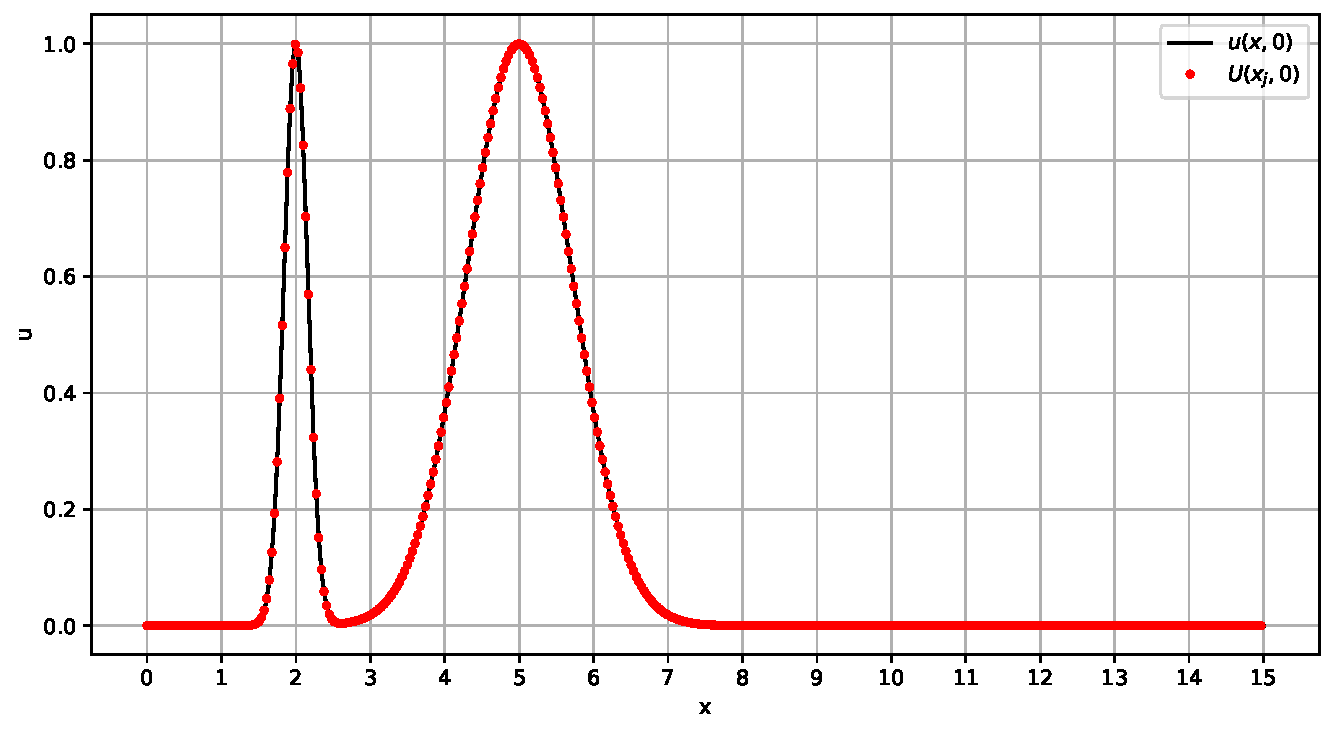
\includegraphics[width=\textwidth]{initial_condition.pdf}
        \caption{Condição inicial.}\label{fig:initial}
    \end{figure}

    \begin{figure}[H]
        \centering

        \begin{subfigure}{0.45\textwidth}
            \centering
            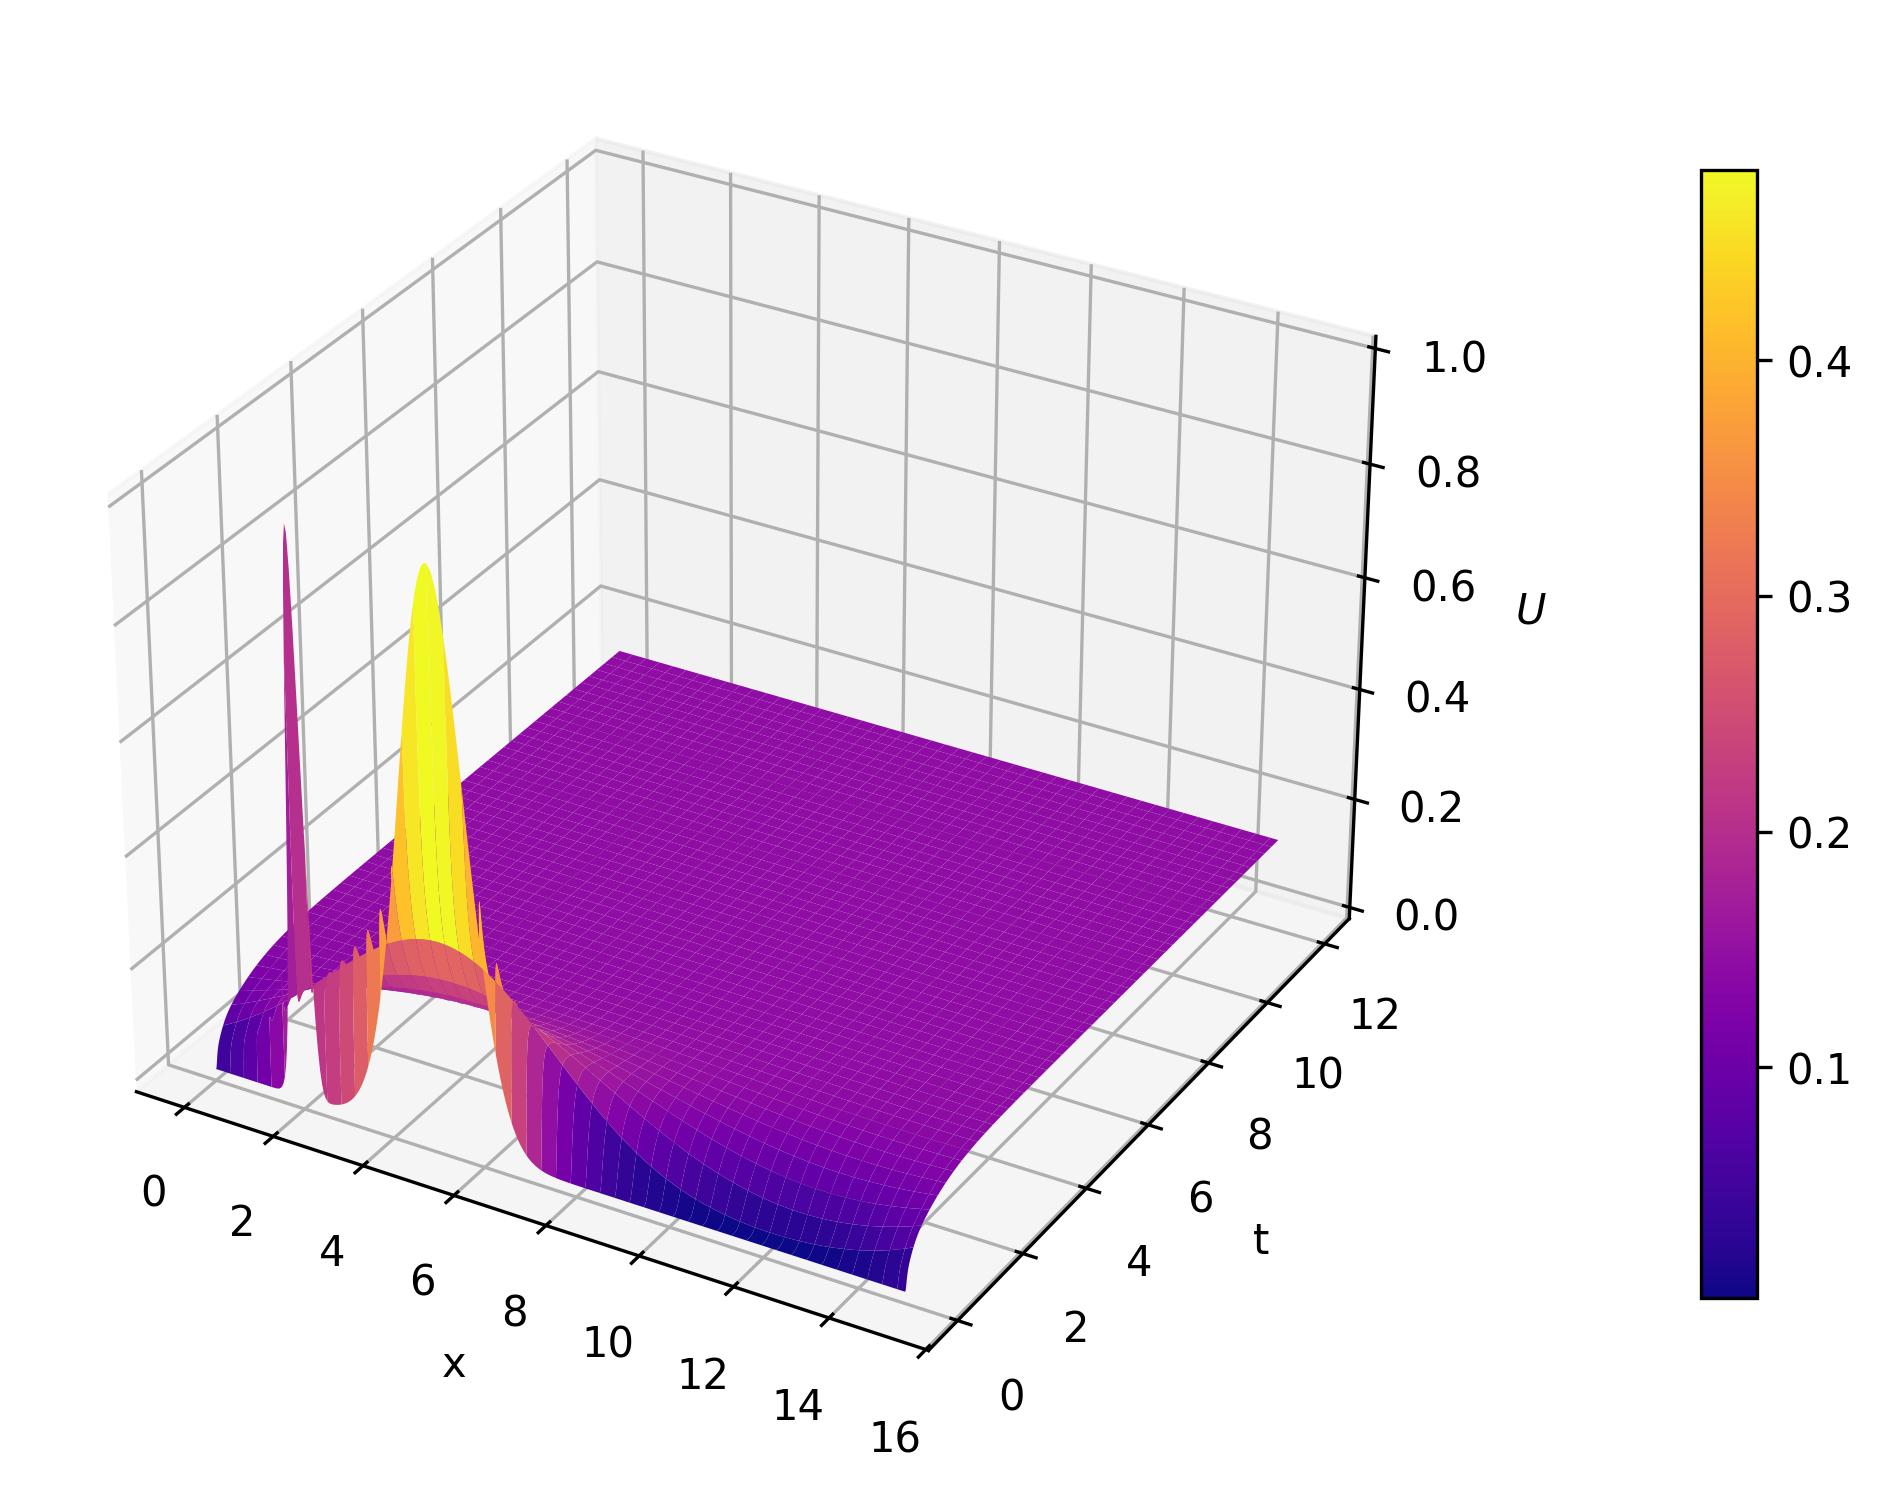
\includegraphics[width=0.85\textwidth]{surface_central_Pe=0.1.png}
            \caption{Solução numérica para $\bb{P}e = 0{,}1 \ll 1$\\(regime de difusão dominante).}\label{fig:Pe0.1}
        \end{subfigure}
        \hfill
        \begin{subfigure}{0.45\textwidth}
            \centering
            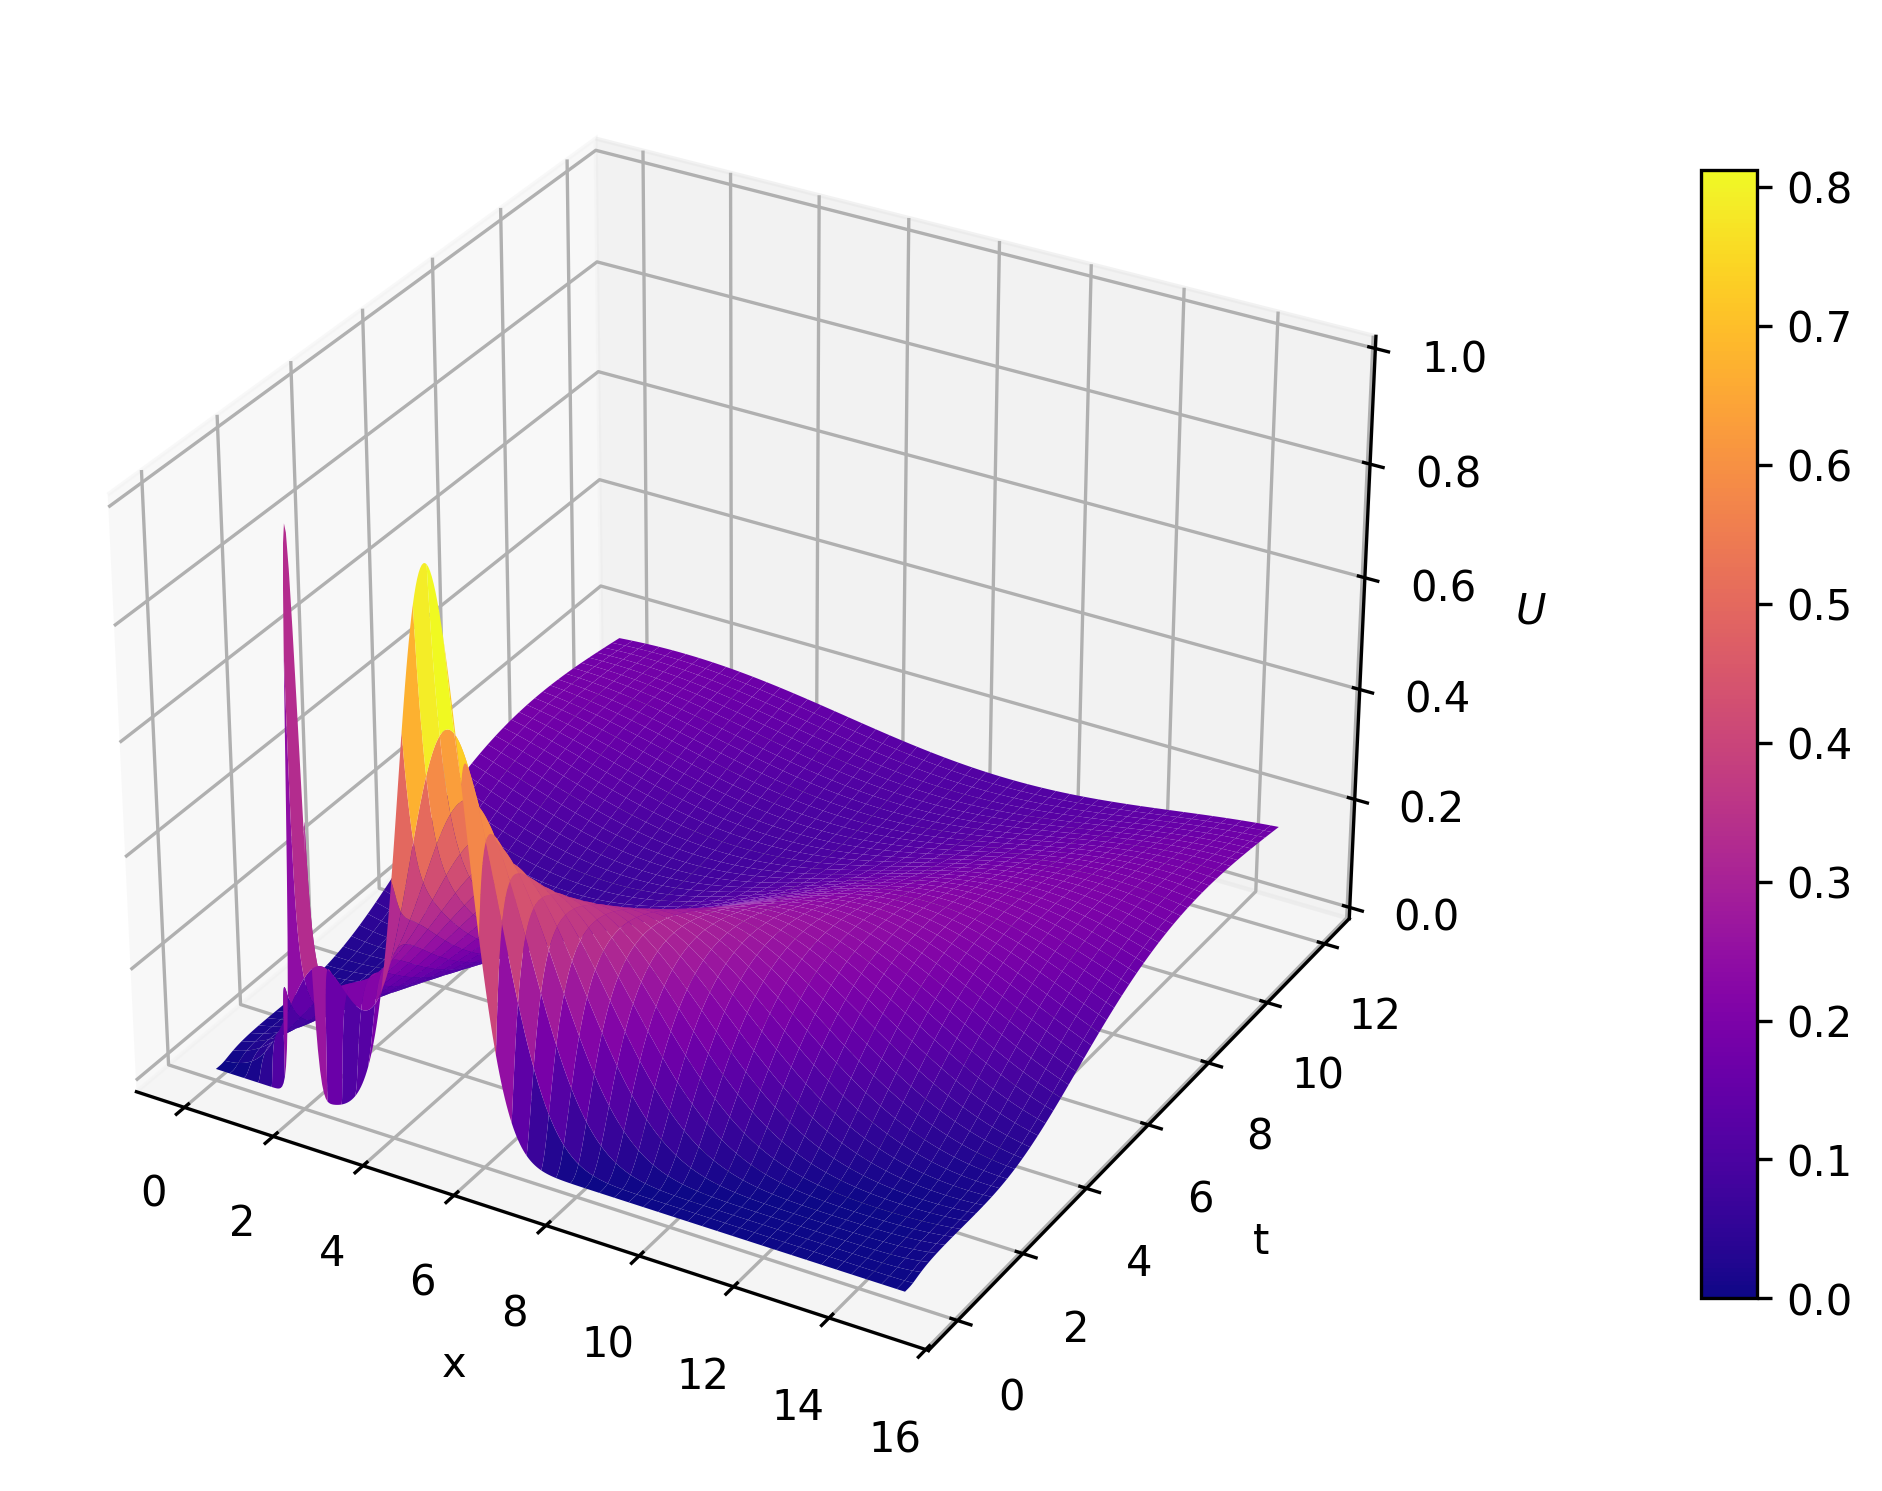
\includegraphics[width=0.85\textwidth]{surface_central_Pe=1.png}
            \caption{Solução numérica para $\bb{P}e = 1$\\(regime de advecção-difusão balanceados).}\label{fig:Pe1}
        \end{subfigure}

        \vspace{0.5cm}

        \begin{subfigure}{0.45\textwidth}
            \centering
            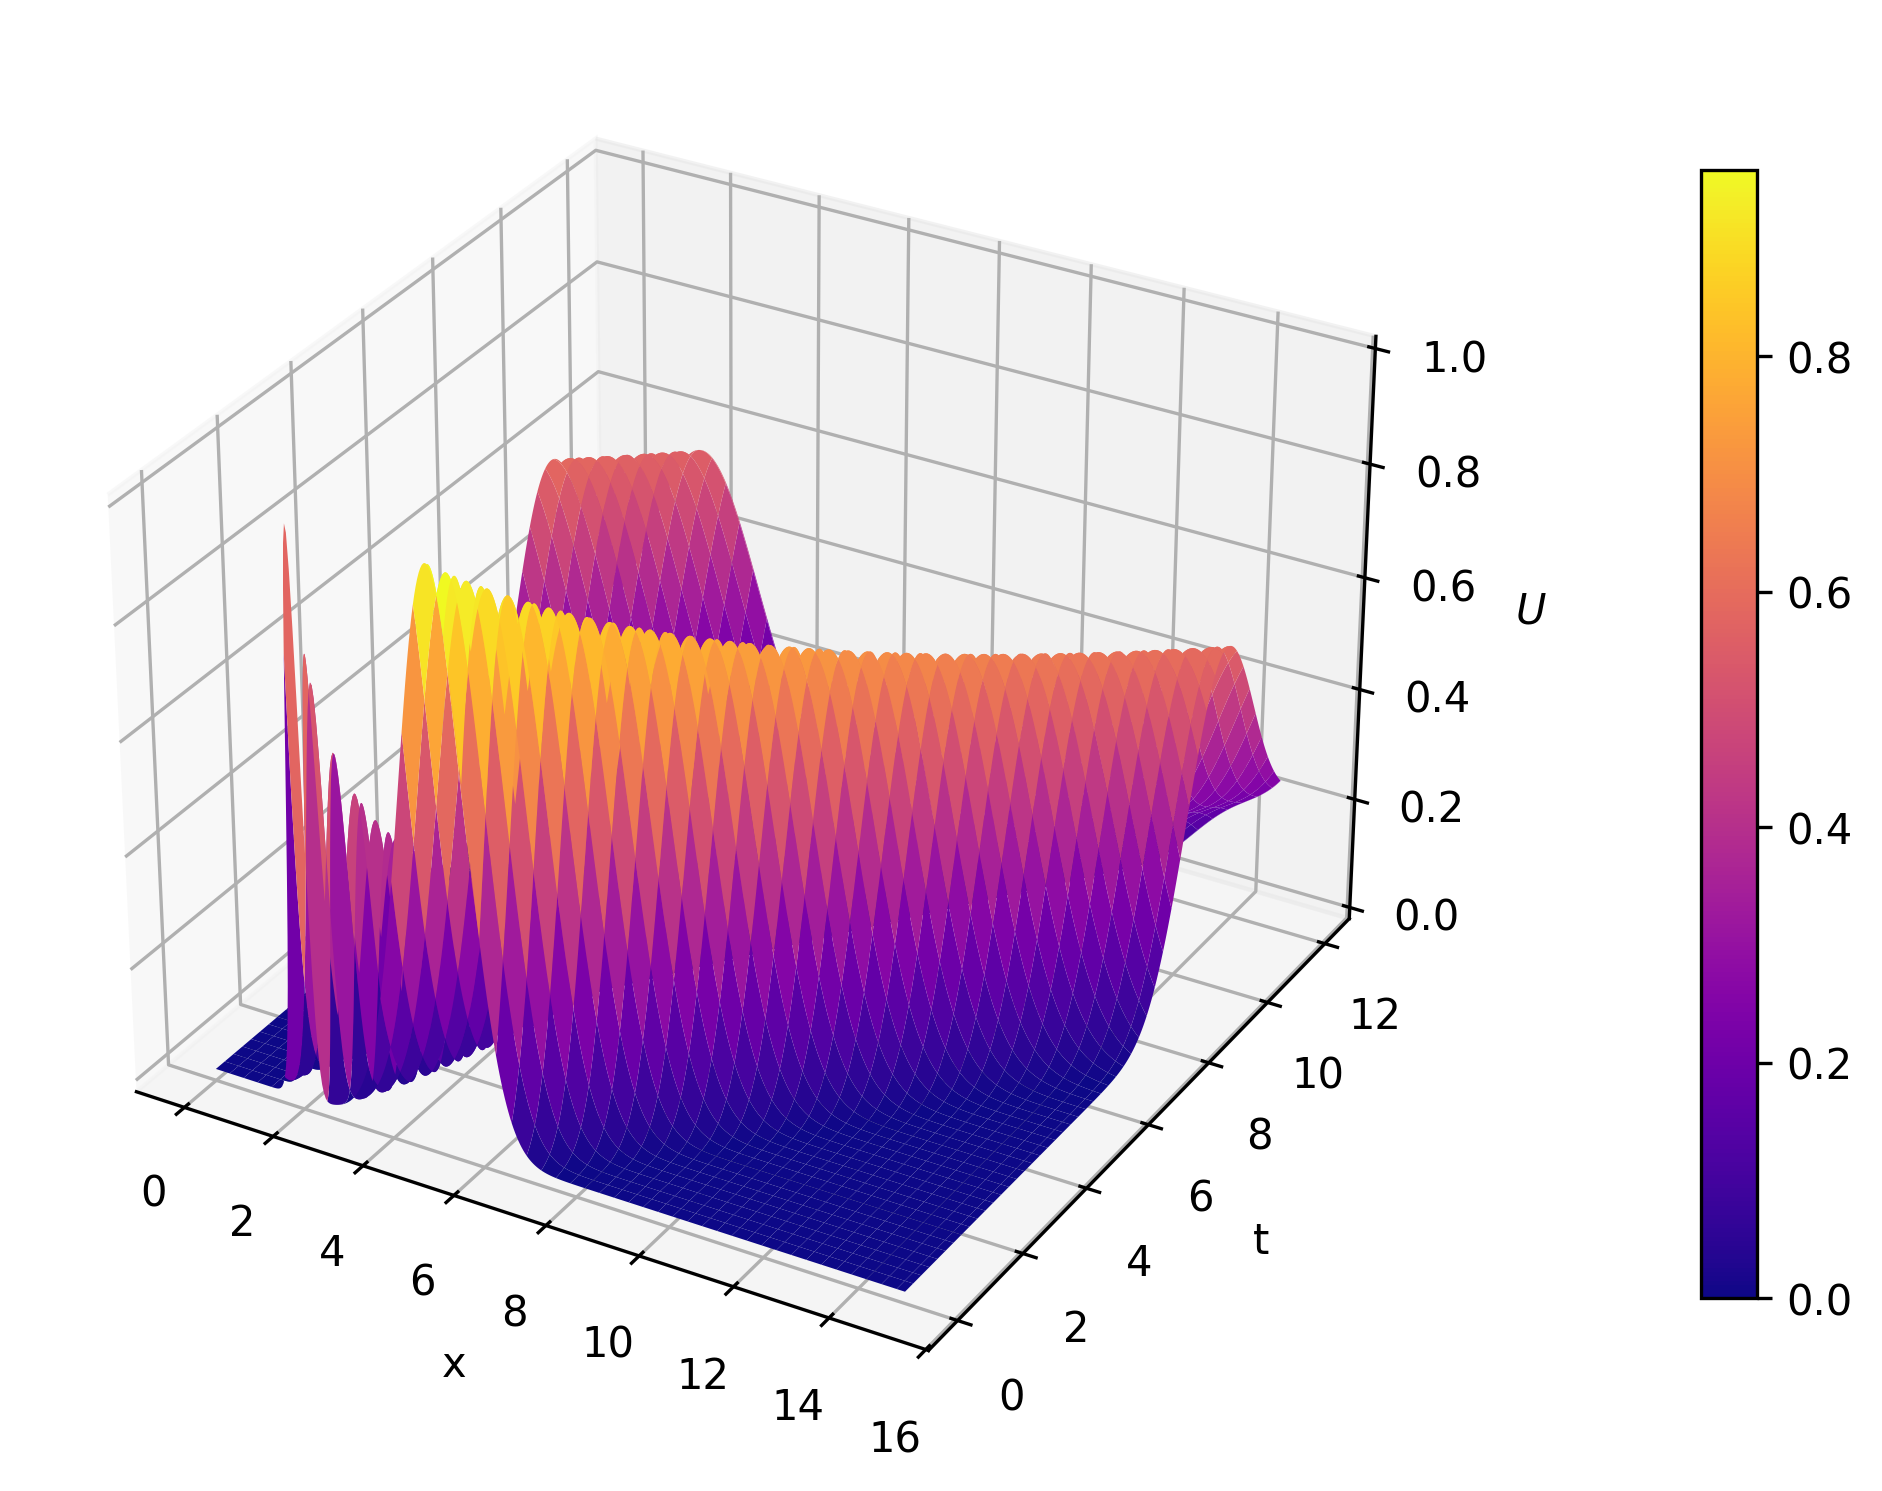
\includegraphics[width=0.85\textwidth]{surface_central_Pe=20.png}
            \caption{Solução numérica para $\bb{P}e = 20 \gg 1$\\(regime de advecção dominante).}\label{fig:Pe20}
        \end{subfigure}

        \caption{Soluções numéricas com o esquema central para valores crescentes de $\Pe$.}\label{fig:central}
    \end{figure}

    \subsection{Diferenças progressivas no tempo e \textit{upwind} no espaço}

    Dado que o coeficiente do termo advectivo é positivo, o esquema \textit{upwind} emprega diferenças regressivas para a primeira derivada espacial, resultando em
    \begin{equation}
        \begin{split}
            &\frac{u(x_j,t_{n+1})-u(x_j,t_n)}{\D{t}} + \O{\D{t}} + \frac{u(x_{j},t_n)-u(x_{j-1},t_n)}{\D{x}} + \O{\D{x}}
            \\&= \frac{1}{\bb{P}e} \frac{u(x_{j+1},t_n)-2u(x_j,t_n)+u(x_{j-1},t_n)}{\D{x}^2} + \O{\D{x}^2},
        \end{split}
    \end{equation}
    o que produz o esquema
    \begin{equation}
        \frac{U_j^{n+1}-U_j^n}{\D{t}} + \frac{U_j^n-U_{j-1}^n}{\D{x}} = \frac{1}{\bb{P}e} \frac{U_{j-1}^n-2U_j^n+U_{j+1}^n}{\D{x}^2},
    \end{equation}
    ou, de forma equivalente,
    \begin{equation}
        \begin{split}
            U_j^{n+1} &= \left(\frac{\D{t}}{\bb{P}e\D{x}^2}+\frac{\D{t}}{\D{x}}\right)U_{j-1}^n + \left(1-\frac{2\D{t}}{\bb{P}e\D{x}^2}-\frac{\D{t}}{\D{x}}\right)U_j^n + \left(\frac{\D{t}}{\bb{P}e\D{x}^2}\right)U_{j+1}^n\\[.2cm]
            &= (\alpha+\gamma)U_{j-1}^n + (1-2\alpha-\gamma)U_j^n + \alpha U_{j+1}^n,
        \end{split}
    \end{equation}
    onde $\alpha = \dfrac{\D{t}}{\bb{P}e\D{x^2}}$ e $\gamma = \dfrac{\D{t}}{\D{x}} = 2\beta$.

    \vspace{.3cm}

    Sob condições de contorno periódicas ($U_{N_x+1}^n = U_0^n$), os nós de fronteira tornam-se:

    $j = 0$:
    \[U_0^{n+1} = (\alpha+\gamma)U_{-1}^n + (1-2\alpha-\gamma)U_0^n + \alpha U_{1}^n = (1-2\alpha-\gamma)U_0^n + \alpha U_{1}^n + (\alpha+\gamma)U_{N_x}^n,\]

    $j = N_x$:
    \[U_{N_x}^{n+1} = (\alpha+\gamma)U_{N_x-1}^n + (1-2\alpha-\gamma)U_{N_x}^n + \alpha U_{N_x+1}^n = \alpha U_{0}^n + (\alpha+\gamma)U_{N_x-1}^n + (1-2\alpha-\gamma)U_{N_x}^n.\]

    A representação matricial do sistema é
    \begin{equation}
        \bf{U^{n+1}} = A\bf{U^n},
    \end{equation}
    onde $\bf{U^n} = \begin{bmatrix}
        U_0^n \\ U_1^n \\ U_2^n \\ \vdots \\ U_{N_x}^n
    \end{bmatrix}$ e $A = \begin{bmatrix}
        (1-2\alpha-\gamma) & \alpha & 0 & \cdots & (\alpha+\gamma)\\
        (\alpha+\gamma) & (1-2\alpha-\gamma) & \alpha & \cdots & 0\\
        0 & (\alpha+\gamma) & (1-2\alpha-\gamma) & \cdots & 0\\
        \vdots & \vdots & \ddots & \ddots & \ddots\\
        \alpha & 0 & \cdots & (\alpha+\gamma) & (1-2\alpha-\gamma)\\
    \end{bmatrix}$.

    \vspace{.4cm}

    A condição inicial discretizada coincide com a do esquema centrado.

    \subsubsection{Análise de Estabilidade}\label{sec:est}

    Pelo critério de Von Neumann, substitui-se $U_j^n = e^{i\omega j}$ no esquema \textit{upwind}, obtendo-se o fator de amplificação $\zeta$ tal que $U_j^{n+1} = \zeta U_j^n$. Substituindo:
    \[\zeta e^{i\omega j} = (\alpha+\gamma) e^{i\omega(j-1)} + (1-2\alpha-\gamma)e^{i\omega j} + \alpha e^{i\omega(j+1)},\]
    \[\begin{split}
        \zeta &= (\alpha+\gamma) e^{-i\omega} + (1-2\alpha-\gamma) + \alpha e^{i\omega}\\
        &= 1 + (e^{-i\omega}+e^{i\omega} - 2)\alpha + (e^{-i\omega} - 1)\gamma\\
        &= 1 + (2\cos(\omega) - 2)\alpha + (\cos(\omega)-i\sin(\omega) - 1)\gamma\\
        &= [1+(2\alpha+\gamma)(\cos(\omega)-1)] - i \gamma\sin(\omega).
    \end{split}\]

    Calculando $|\zeta|^2$:
    \[\begin{split}
        |\zeta|^2 &= {[1+(2\alpha+\gamma)(\cos(\omega)-1)]}^2 + {[\gamma\sin(\omega)]}^2\\
        &= 1 + 2(2\alpha+\gamma)(\cos(\omega)-1) + {(2\alpha+\gamma)}^2{(\cos(\omega)-1)}^2 + \gamma^2\sin^2(\omega)\\
    \end{split}\]
    \[= 1 - 4(2\alpha+\gamma)\sin^2(\omega/2) + {(2\alpha+\gamma)}^2{(-2\sin^2(\omega/2))}^2 + \gamma^2\sin^2(\omega)\]
    \[= 1 - (8\alpha+4\gamma)\sin^2(\omega/2) + (16\alpha^2+16\alpha\gamma+4\gamma^2)\sin^4(\omega/2) + \gamma^2\sin^2(\omega)\]
    \[= 1 - (8\alpha+4\gamma)\sin^2(\omega/2) + (16\alpha^2+16\alpha\gamma+4\gamma^2)\sin^4(\omega/2) + \gamma^2(4\sin^2(\omega/2)-4\sin^4(\omega/2))\]
    \[= 1 - (8\alpha+4\gamma-4\gamma^2)\sin^2(\omega/2) + (16\alpha^2+16\alpha\gamma+4\gamma^2-4\gamma^2)\sin^4(\omega/2)\]
    \[\leq 1 - (8\alpha+4\gamma-4\gamma^2) + (16\alpha^2+16\alpha\gamma).\]

    Portanto, $|\zeta|^2 \leq 1$ se e somente se $-(8\alpha+4\gamma-4\gamma^2) + (16\alpha^2+16\alpha\gamma) \leq 0$, o que se reduz a
    \[\begin{split}
        -8\alpha-4\gamma+4\gamma^2 + 16\alpha^2+16\alpha\gamma &\leq 0\\
        -(2\alpha+\gamma)+{(2\alpha+\gamma)}^2 &\leq 0\\
        (2\alpha+\gamma)(2\alpha+\gamma-1) &\leq 0.
    \end{split}\]

    Como $\alpha,\gamma > 0$, tem-se $2\alpha+\gamma > 0$, de modo que a condição de estabilidade equivale a
    \[\begin{split}
        2\alpha+\gamma -1 &\leq 0\\
        2\alpha+\gamma &\leq 1\\
        2\dfrac{\D{t}}{\bb{P}e\D{x^2}} + \dfrac{\D{t}}{\D{x}} &\leq 1\\
        \therefore \D{t} &\leq \dfrac{\D{x^2}}{\frac{2}{\bb{P}e}+\D{x}}.
    \end{split}\]

    \section{Impacto do Número de Péclet na Discretização}\label{sec:peclet}

    A restrição $\Delta t < \min\left\{ \dfrac{\Delta x^2}{\frac{2}{\bb{P}e} + \Delta x}, \Delta x \right\}$ decorre da análise de estabilidade do esquema \textit{upwind} combinada com a condição CFL $\frac{\D{t}}{\D{x}} < 1$. Como $\Pe > 0$, verifica-se que
    \begin{align}
        \frac{\Delta x^2}{\frac{2}{\bb{P}e}+ \D{x}} < \frac{\Delta x^2}{\D{x}} = \D{x}, \notag
    \end{align}
    de forma que a restrição efetiva se reduz a $\Delta t < \dfrac{\Delta x^2}{\frac{2}{\bb{P}e} + \Delta x}$.

    \vspace{.2cm}

    Analisando os coeficientes $\alpha$ e $\beta$ da equação~\eqref{eq:centradas} com $\D{t}$ dado por~\eqref{eq:dt}, obtêm-se os seguintes comportamentos assintóticos:

    Para $\Pe \gg 1$:
    \begin{align}
        \D{t} = \frac{(1-\varepsilon)\D{x^2}}{\frac{2}{\Pe} + \D{x}} &\approx (1-\varepsilon) \D{x}, \notag \\
        \alpha = \frac{\D{t}}{\Pe \D{x^2}} &\approx \frac{(1-\varepsilon)}{\Pe \D{x}} \ll \frac{1}{\D{x}}, \notag \\
        \beta = \frac{\D{t}}{2 \D{x}} &\approx \frac{(1- \varepsilon)}{2}. \notag
    \end{align}

    Para $\Pe \ll 1$:
    \begin{align}
        \D{t} = \frac{\Pe (1-\varepsilon)\D{x^2}}{2 + \Pe \D{x}} &\approx \frac{\Pe (1-\varepsilon)\D{x^2}}{2}, \notag \\
        \alpha = \frac{\D{t}}{\Pe \D{x^2}} &\approx \frac{(1-\varepsilon)}{2}, \notag \\
        \beta = \frac{\D{t}}{2 \D{x}} &\approx \frac{\Pe(1-\varepsilon)\D{x}}{4} \ll \frac{\D{x}}{4}. \notag
    \end{align}

    \subsection{Discretização Centrada}

    No regime $\Pe \gg 1$, tem-se $\alpha \approx 0$, e a equação~\eqref{eq:centradas} se aproxima de
    \[
        U_j^{n+1} \approx \beta U_{j-1}^n + U_j^n -\beta U_{j+1}^n = U_j^n + \frac{\D{t}}{2\D{x}}(U_{j-1}^n - U_{j+1}^n),
    \]
    que é consistente com a equação puramente advectiva $u_t + u_x = 0$. Contudo, esse esquema é incondicionalmente instável para a equação de advecção pura, conforme pode ser demonstrado pela análise de Von Neumann. Portanto, ao crescer $\Pe$, a discretização centrada tende à instabilidade, o que é investigado na Seção~\ref{sec:inst}.

    No regime $\Pe \ll 1$, tem-se $\beta \approx 0$, e o esquema se reduz a
    \[
        U_j^{n+1} \approx \alpha U_{j-1}^n + (1 - 2\alpha) U_{j}^n + \alpha U_{j+1}^n = U_{j}^n + \frac{1}{\Pe}\frac{\D{t}}{\D{x^2}}(U_{j-1}^n - 2 U_{j}^n + U_{j-1}^n),
    \]
    consistente com a equação de difusão pura $u_t = \frac{1}{\Pe} u_{xx}$, condicionalmente estável.

    \subsubsection{Instabilidade para Número de Péclet Elevado}\label{sec:inst}

    A região de estabilidade do esquema centrado é determinada analogamente à Seção~\ref{sec:est}. O fator de amplificação satisfaz
    \begin{equation}
        \begin{split}
            \zeta &= 1 + 2\alpha(\cos(\omega) - 1) - 2i\beta\sin(\omega) \\
                  &= 1 - 4\alpha\sin^2\left(\frac{\omega}{2}\right) - 2i\beta\sin(\omega).
        \end{split}
    \end{equation}

    Definindo $s = \sin^2\left( \frac{\omega}{2} \right) \in [0,1]$ e notando que $\sin^2(\omega) = 4s(1-s)$, obtém-se
    \begin{equation}
        |\zeta|^2 = 1-8\alpha s + 16\alpha^2 s^2 + 16\beta^2 s(1-s).
    \end{equation}

    A condição $|\zeta|^2 \leq 1$ exige que
    \begin{equation}
        2s^2 (\alpha^2 - \beta^2) + s(2\beta^2 - \alpha) \leq 0, \quad \forall s \in [0,1].
    \end{equation}

    Dividindo por $s > 0$ e impondo a desigualdade nos extremos do intervalo, obtêm-se as condições $2\beta^2 \leq \alpha$ (para $s \to 0^+$) e $\alpha \leq \frac{1}{2}$ (para $s = 1$), que em termos de $\D{t}$, $\D{x}$ e $\Pe$ equivalem a
    \begin{equation}
        \D{t} < \min\left\{\frac{\Pe\D{x^2}}{2}, \frac{2}{\Pe} \right\}.
    \end{equation}

    Verifica-se que, se $\D{t}$ satisfaz a restrição de estabilidade do esquema \textit{upwind},
    \[
        \Delta t < \frac{\Pe \D{x^2}}{2 + \Pe \D{x}} < \frac{\Pe \D{x^2}}{2},
    \]
    e se adicionalmente $\D{x} \leq \frac{2}{\Pe}$, então
    \[
        \D{t} < \frac{\Pe \D{x^2}}{\Pe \D{x}} = \D{x} \leq \frac{2}{\Pe}.
    \]
    Portanto, para malha espacial fixada, o esquema centrado se torna instável à medida que $\Pe$ cresce, pois a região de estabilidade se contrai progressivamente e o fator de amplificação pode facilmente excedê-la. Esse comportamento é evidenciado nas Figuras~\ref{fig:instabilidade}, em que para $\Pe$ suficientemente grande a solução diverge com erros da ordem de $10^{32}$.

    \begin{figure}[H]
        \centering

        \begin{subfigure}{0.45\textwidth}
            \centering
            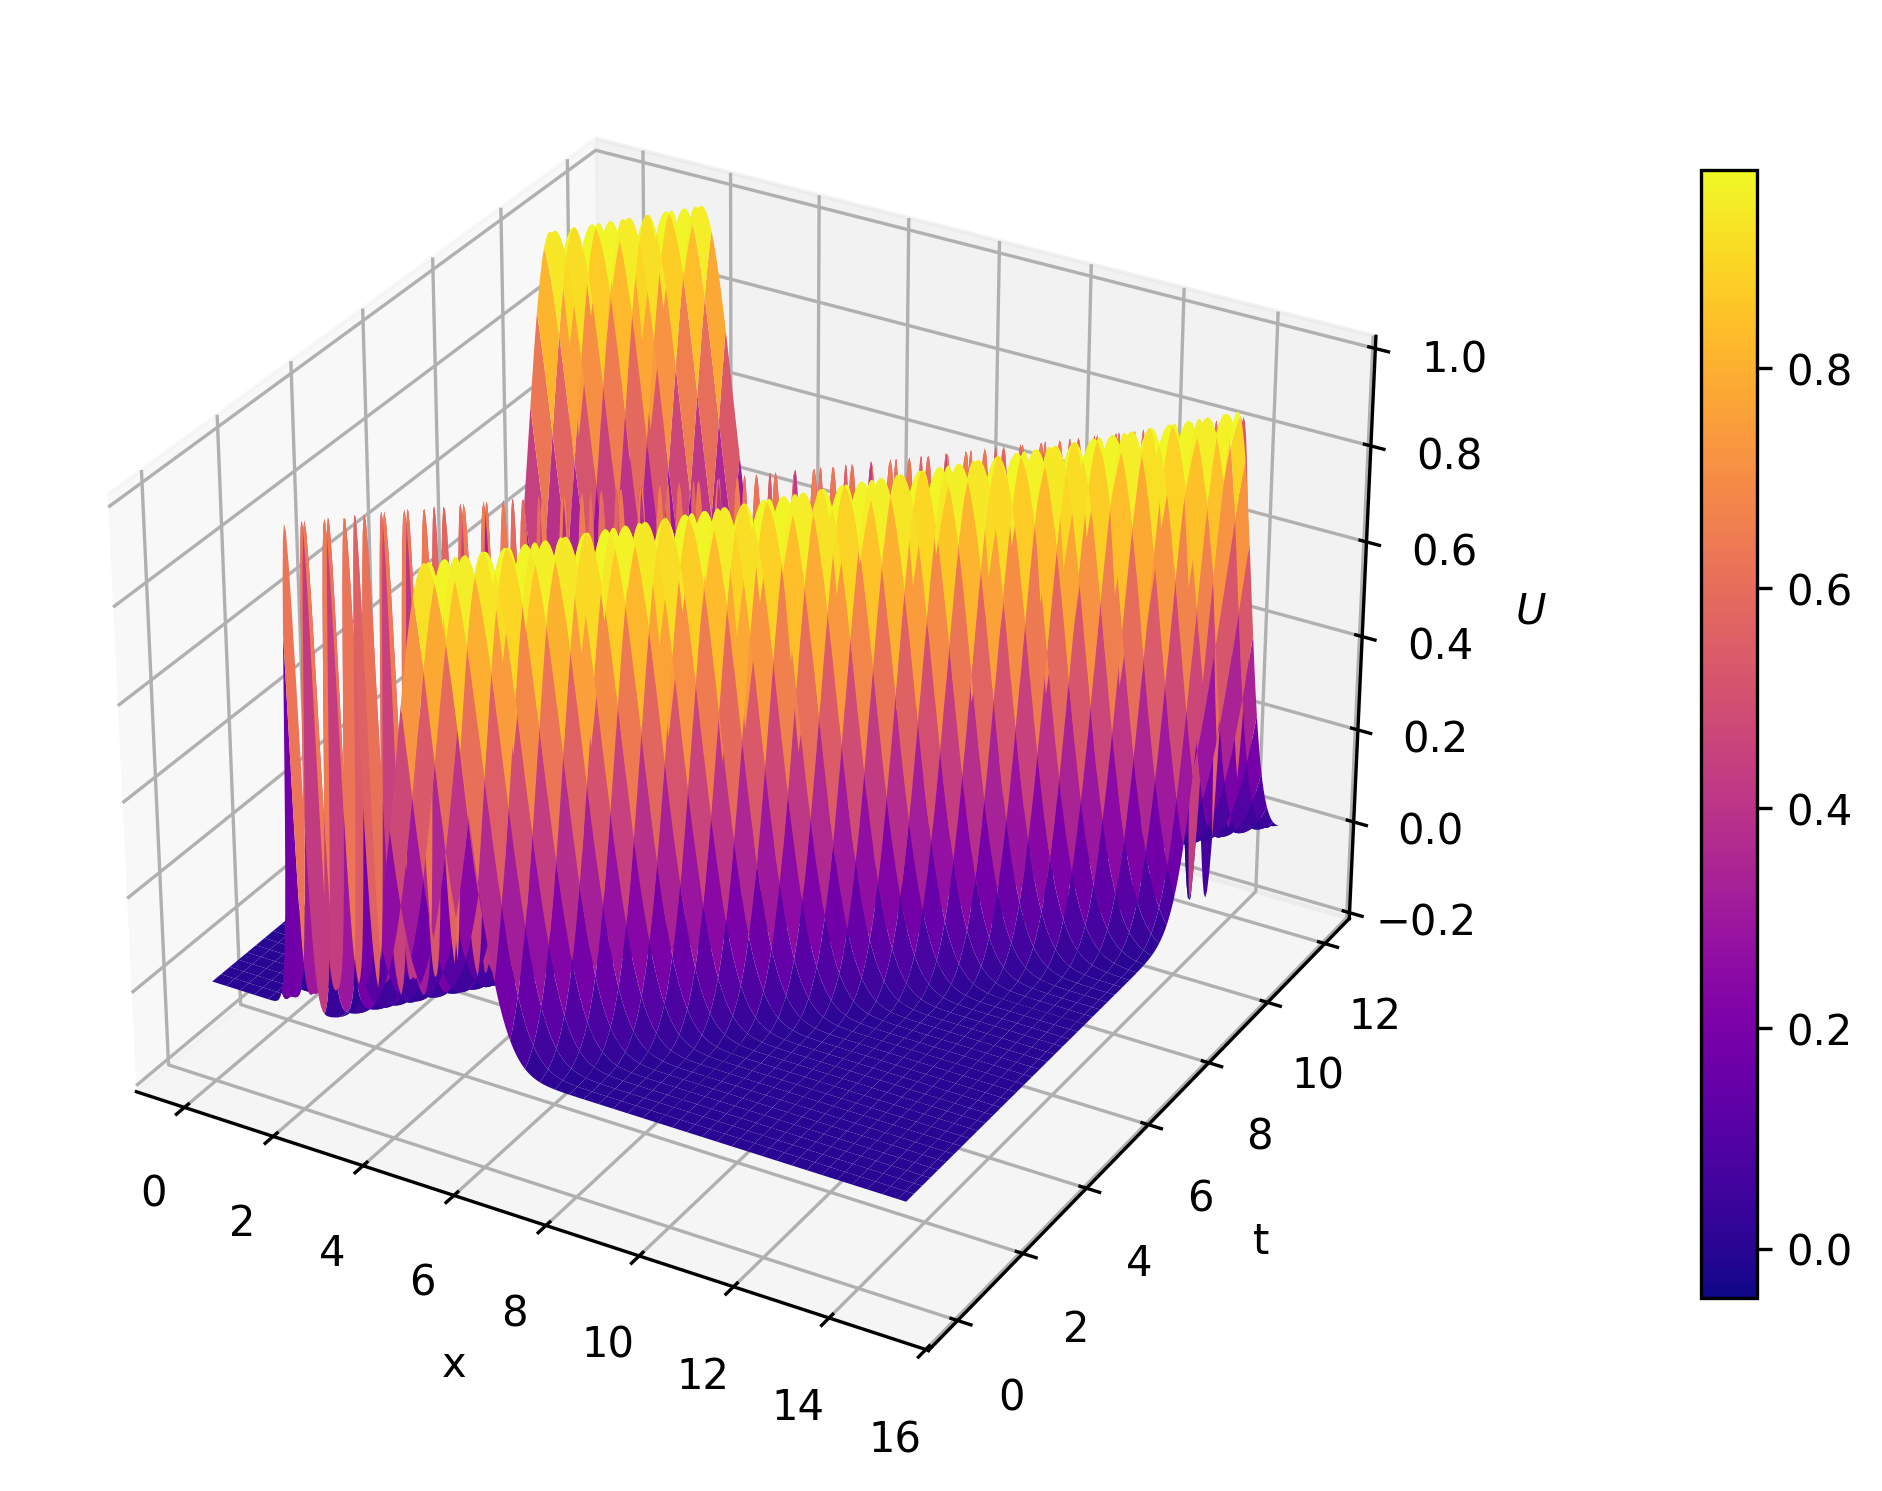
\includegraphics[width=\linewidth]{surface_central_Pe=100.png}
            \caption{Solução numérica para $\bb{P}e = 100$.}\label{fig:Pe100}
        \end{subfigure}
        \hfill
        \begin{subfigure}{0.45\textwidth}
            \centering
            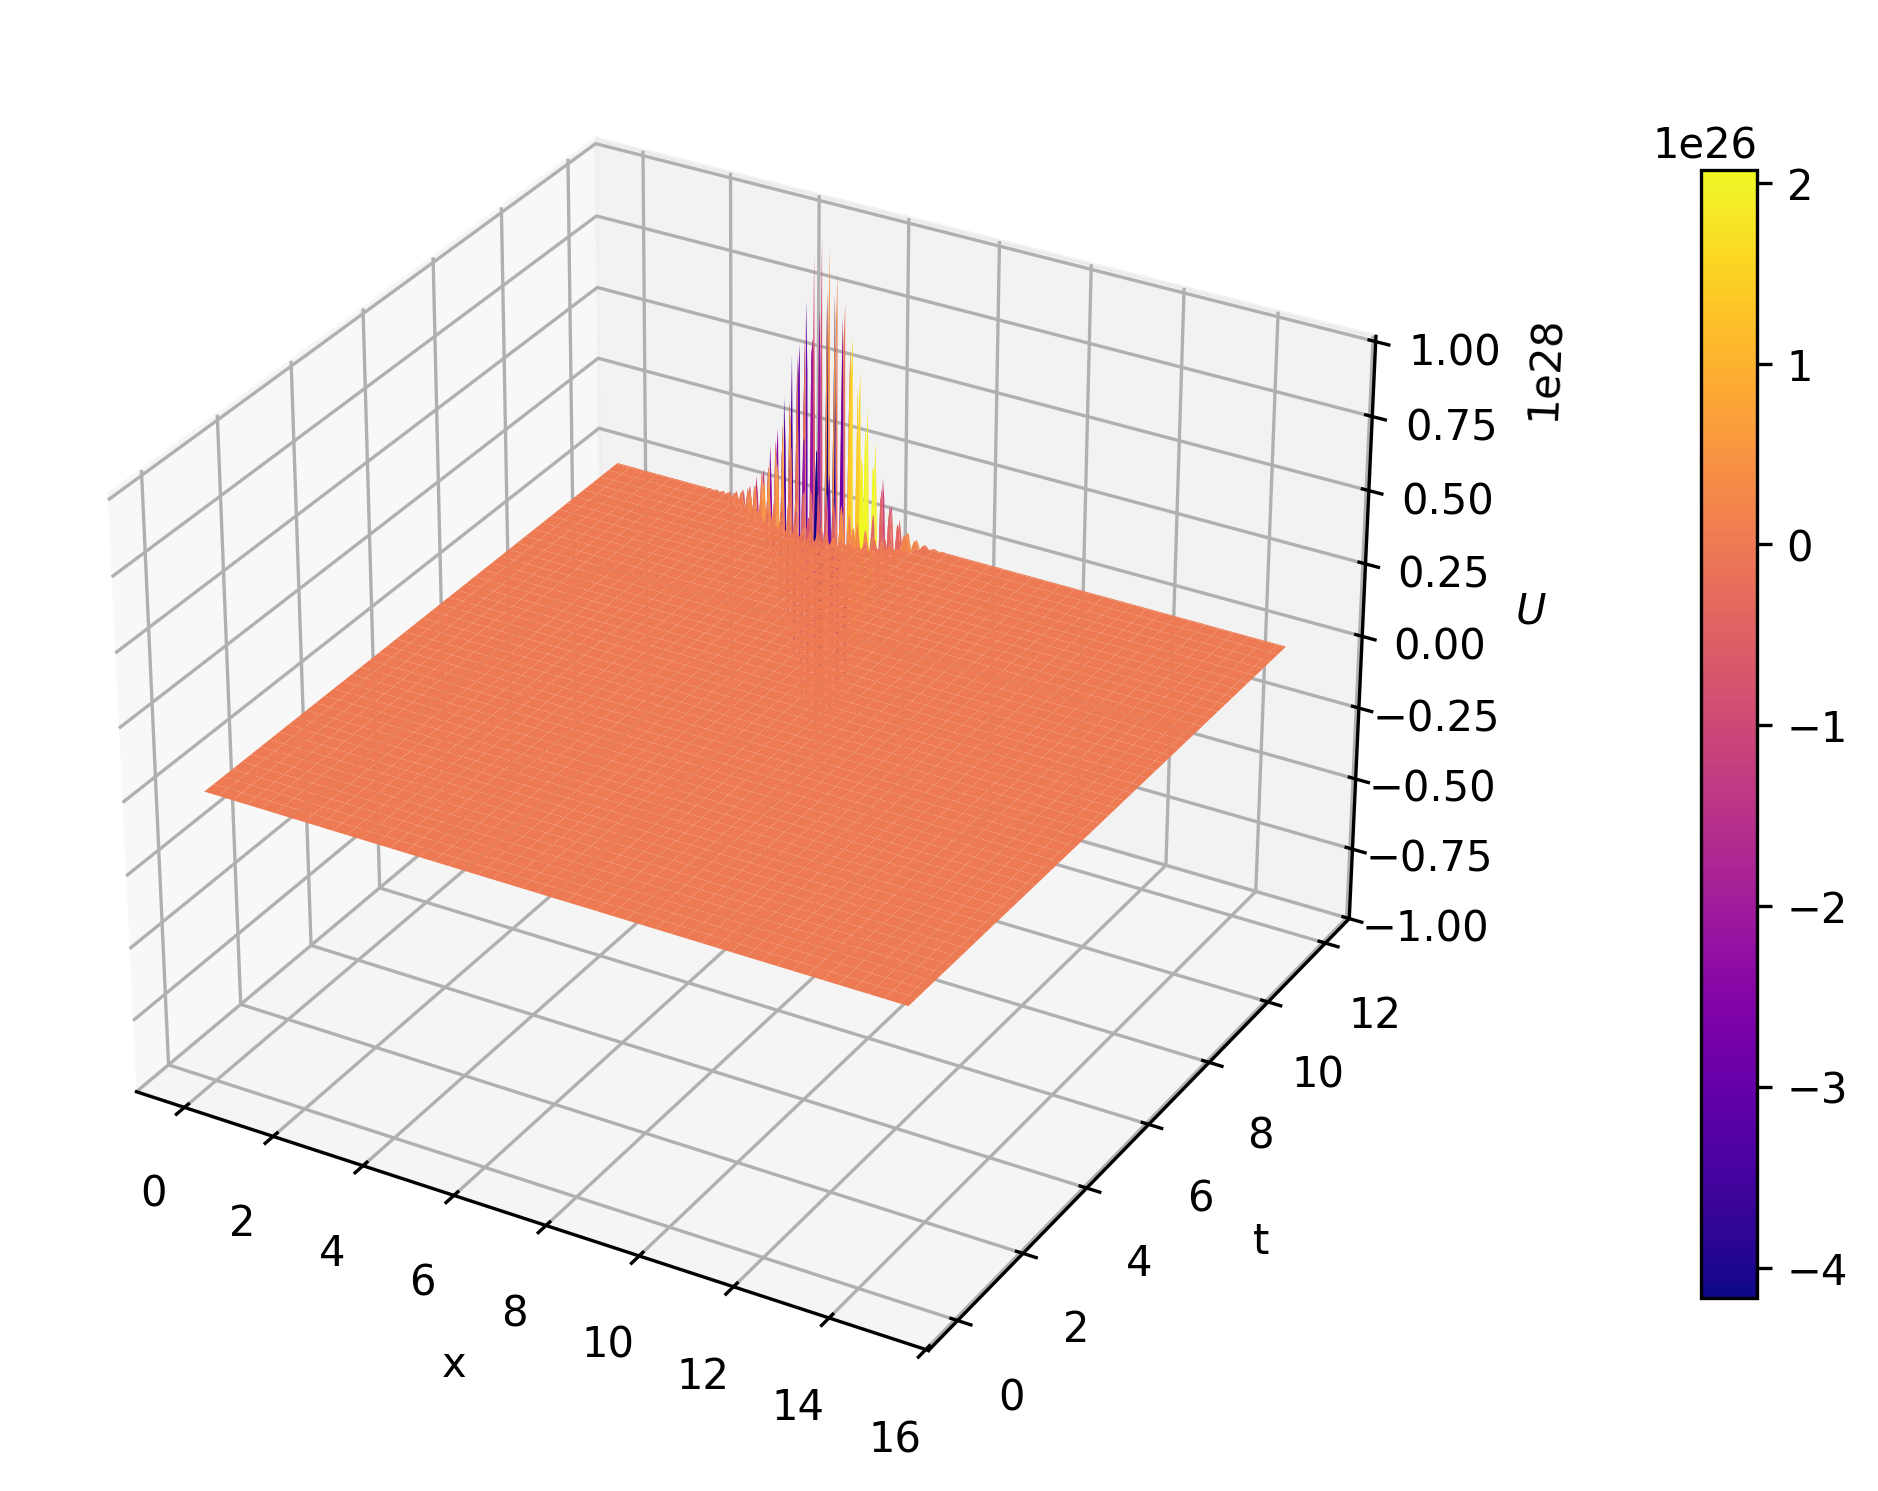
\includegraphics[width=\linewidth]{surface_central_Pe=500.png}
            \caption{Solução numérica para $\bb{P}e = 500$.}\label{fig:Pe500}
        \end{subfigure}

        \vspace{0.5cm}

        \begin{subfigure}{0.45\textwidth}
            \centering
            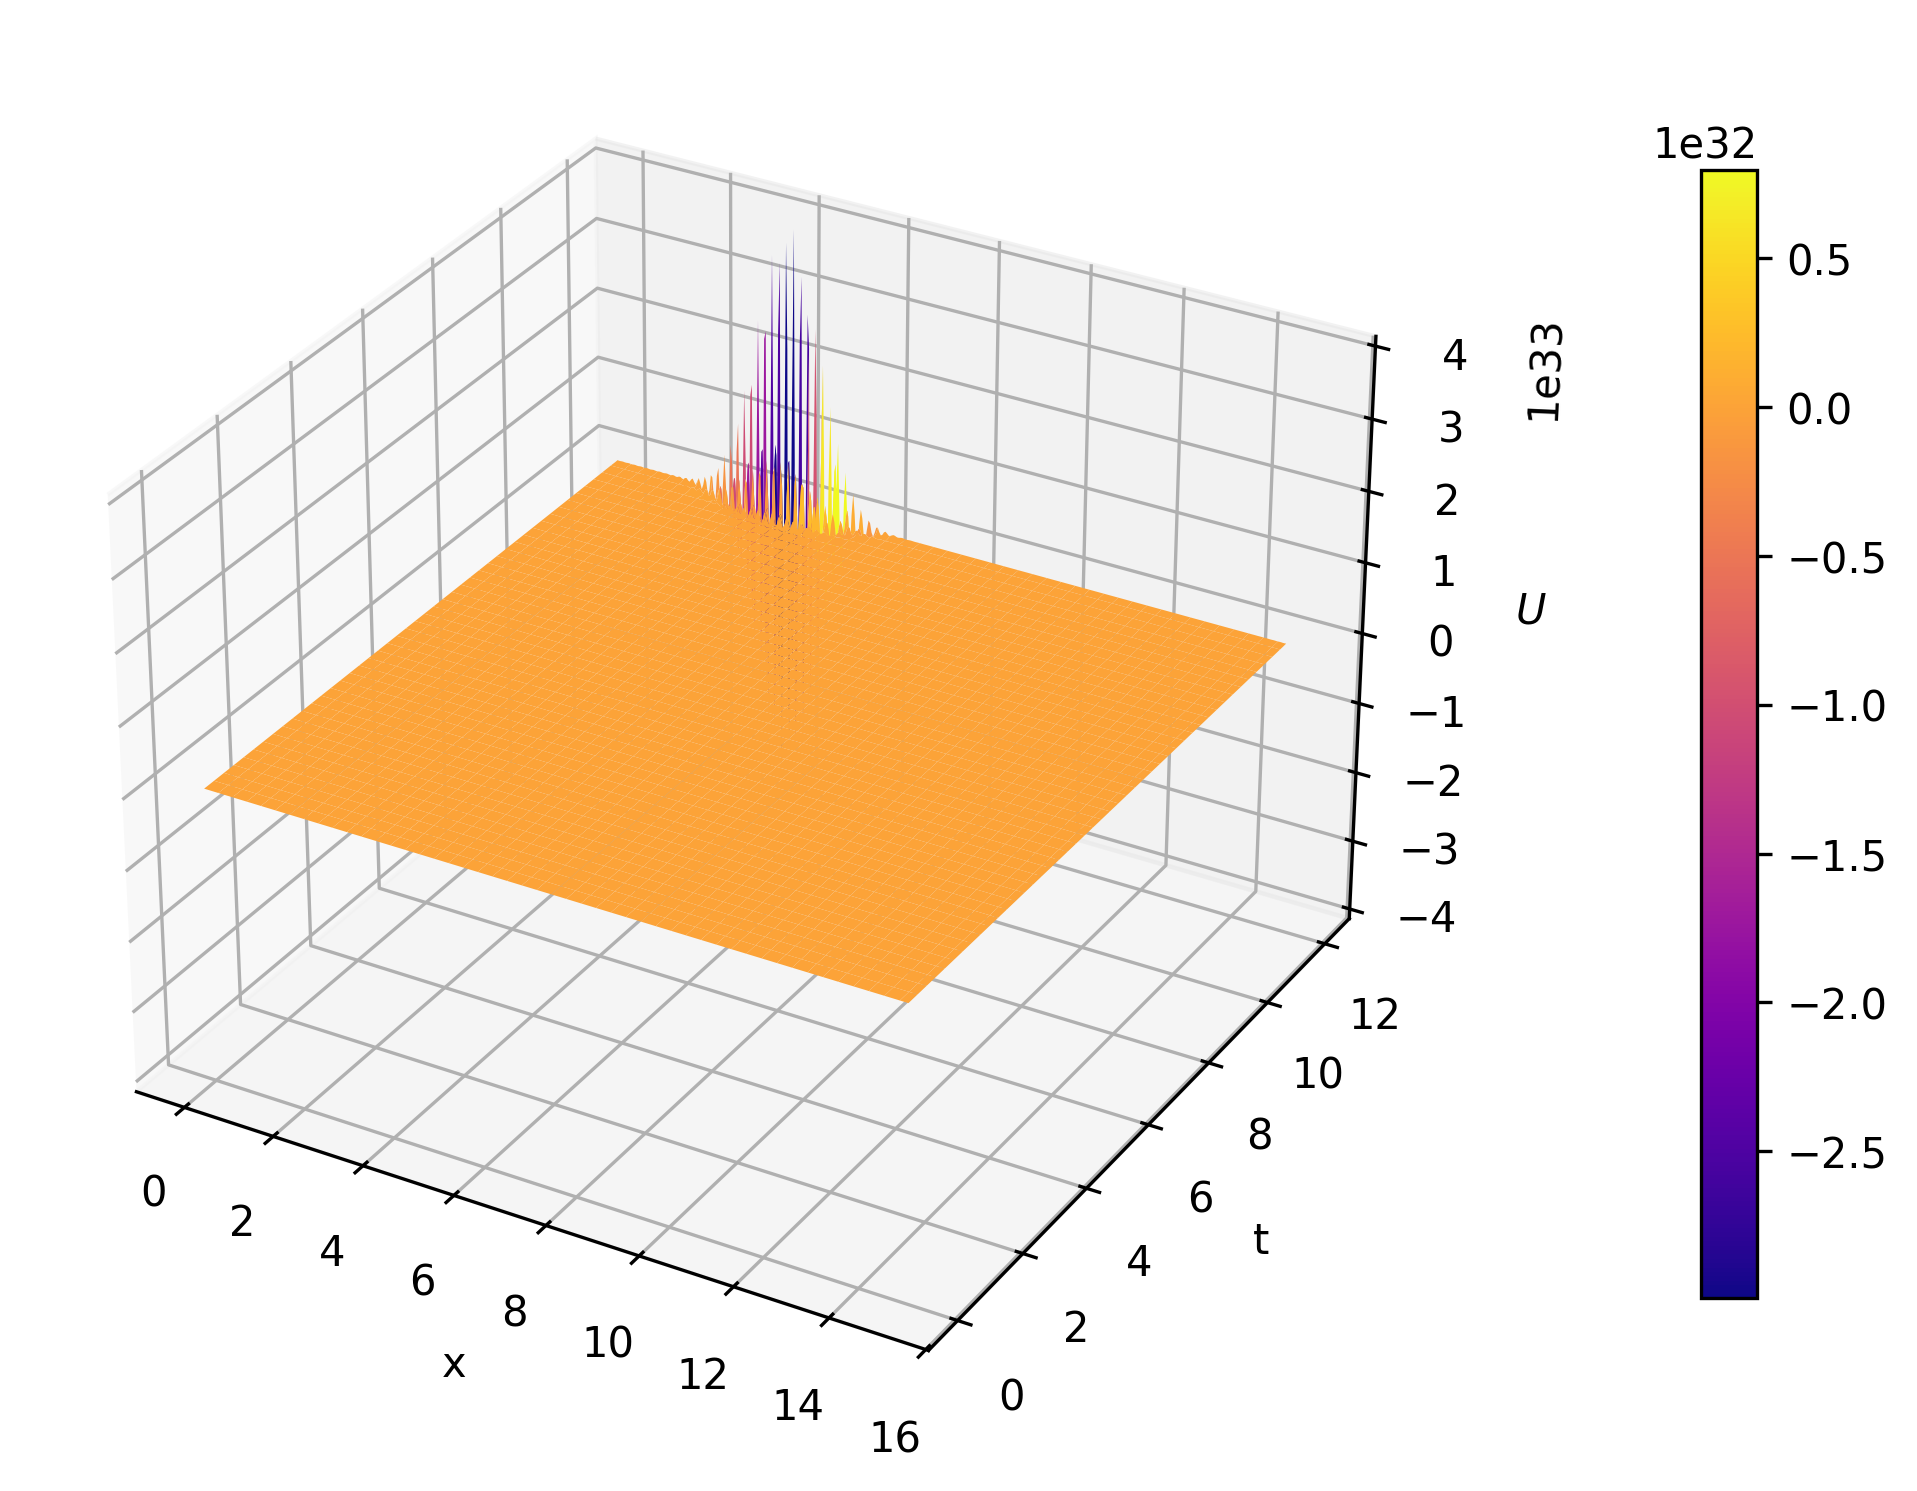
\includegraphics[width=\linewidth]{surface_central_Pe=1000.png}
            \caption{Solução numérica para $\bb{P}e = 1000$.}\label{fig:Pe1000}
        \end{subfigure}

        \caption{Instabilidade numérica do esquema centrado para valores crescentes de $\Pe$.}\label{fig:instabilidade}
    \end{figure}

    \subsection{Esquema \textit{Upwind}}

    Recordando que $\gamma = 2\beta$, para $\Pe \gg 1$ o esquema \textit{upwind} se aproxima de
    \[
        U_j^{n+1} \approx \gamma U_{j-1}^n + (1 - \gamma)U_j^n = U_j^n -\frac{\D{t}}{\D{x}} (U_j^n - U_{j-1}^n),
    \]
    que é consistente com a equação advectiva pura e estável sob a condição CFL{.}

    Para $\Pe \ll 1$, o esquema se reduz a
    \[
        U_j^{n+1} \approx \alpha U_{j-1}^n + (1-2\alpha)U_j^n + \alpha U_{j+1}^n = U_{j}^n + \frac{1}{\Pe}\frac{\D{t}}{\D{x^2}}(U_{j-1}^n - 2 U_{j}^n + U_{j-1}^n),
    \]
    coincidindo com o comportamento assintótico do esquema centrado nesse regime.

    Ao contrário da discretização centrada, o esquema \textit{upwind} não apresenta instabilidade numérica com o crescimento de $\Pe$, uma vez que recupera o próprio método \textit{upwind} puro no limite $\Pe \to \infty$. Esse comportamento é ilustrado nas Figuras~\ref{fig:upwind}.

    \begin{figure}[H]
        \centering

        \begin{subfigure}{0.45\textwidth}
            \centering
            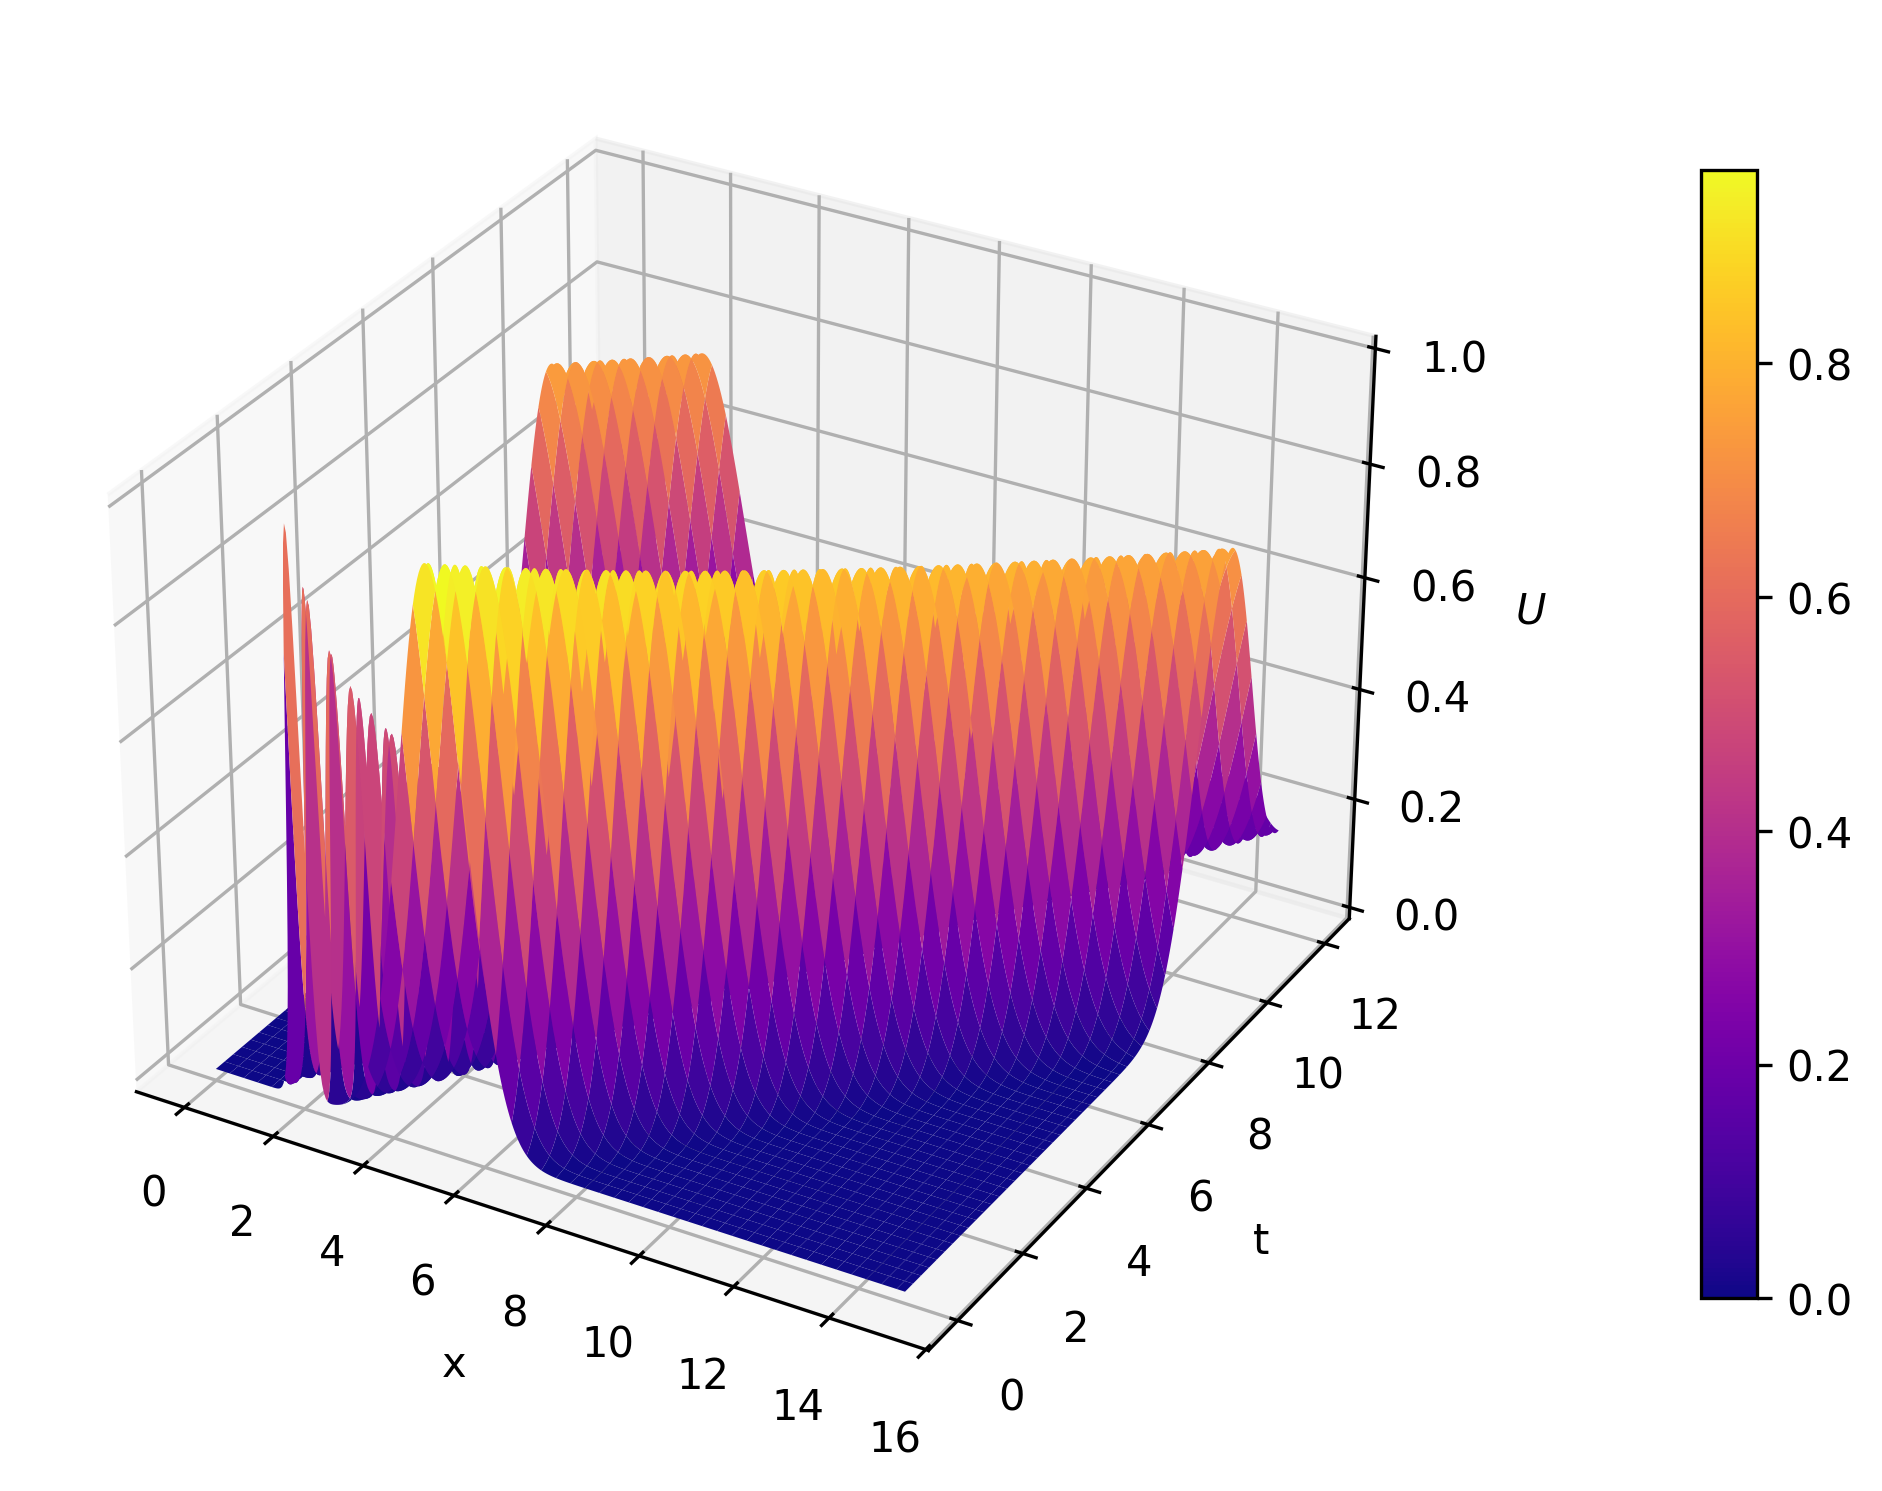
\includegraphics[width=\linewidth]{surface_upwind_Pe=100.png}
            \caption{Solução com \textit{upwind} para $\bb{P}e = 100$.}\label{fig:Pe100up}
        \end{subfigure}
        \hfill
        \begin{subfigure}{0.45\textwidth}
            \centering
            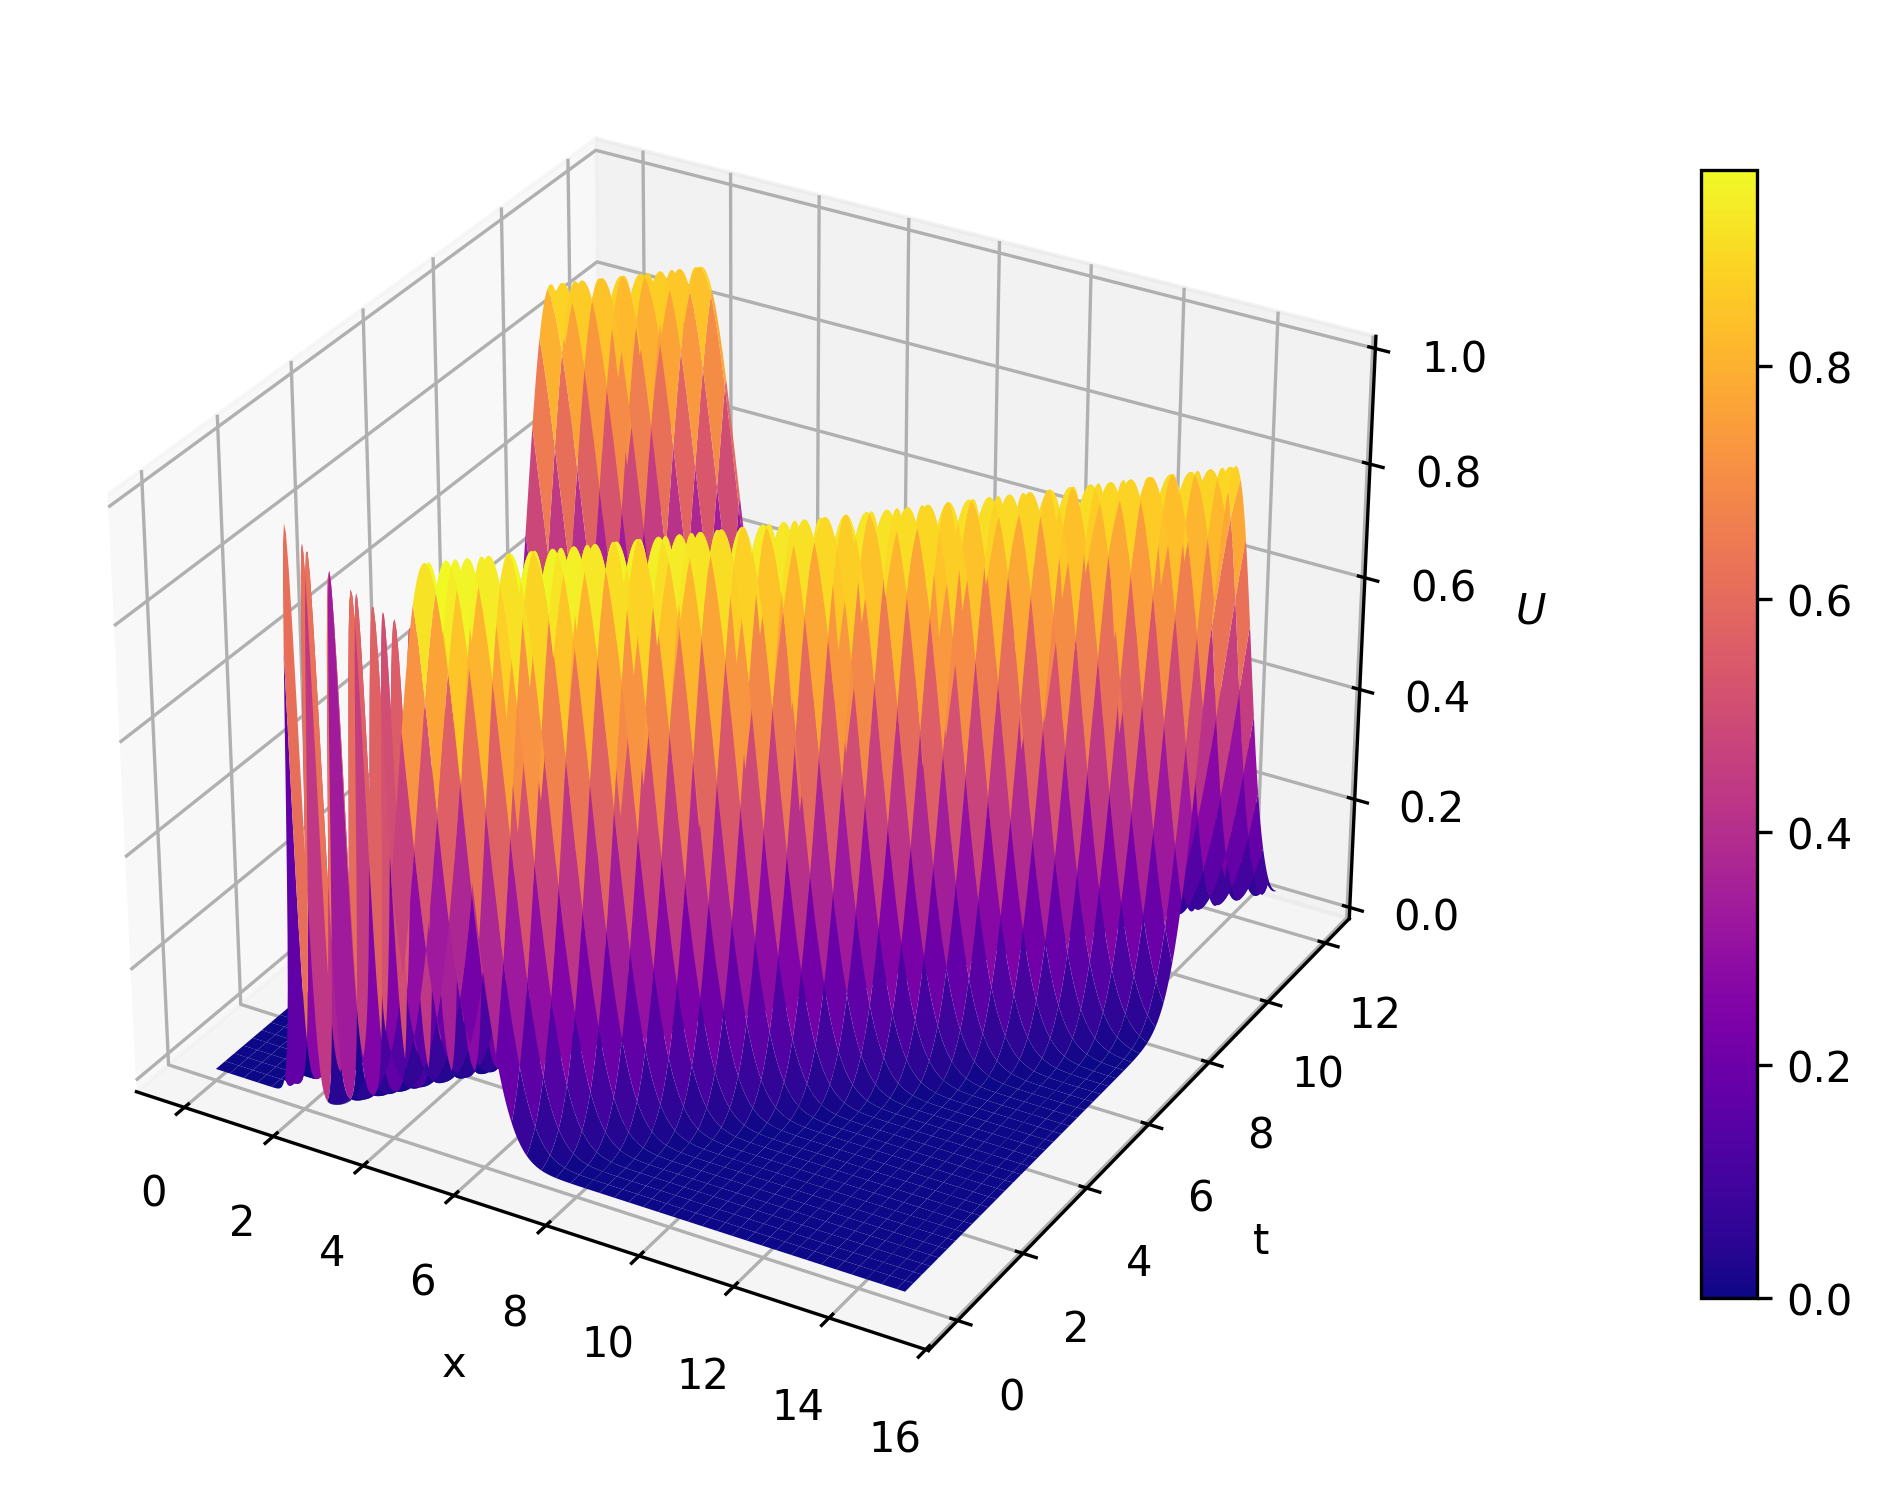
\includegraphics[width=\linewidth]{surface_upwind_Pe=500.png}
            \caption{Solução com \textit{upwind} para $\bb{P}e = 500$.}\label{fig:Pe500up}
        \end{subfigure}

        \vspace{0.5cm}

        \begin{subfigure}{0.45\textwidth}
            \centering
            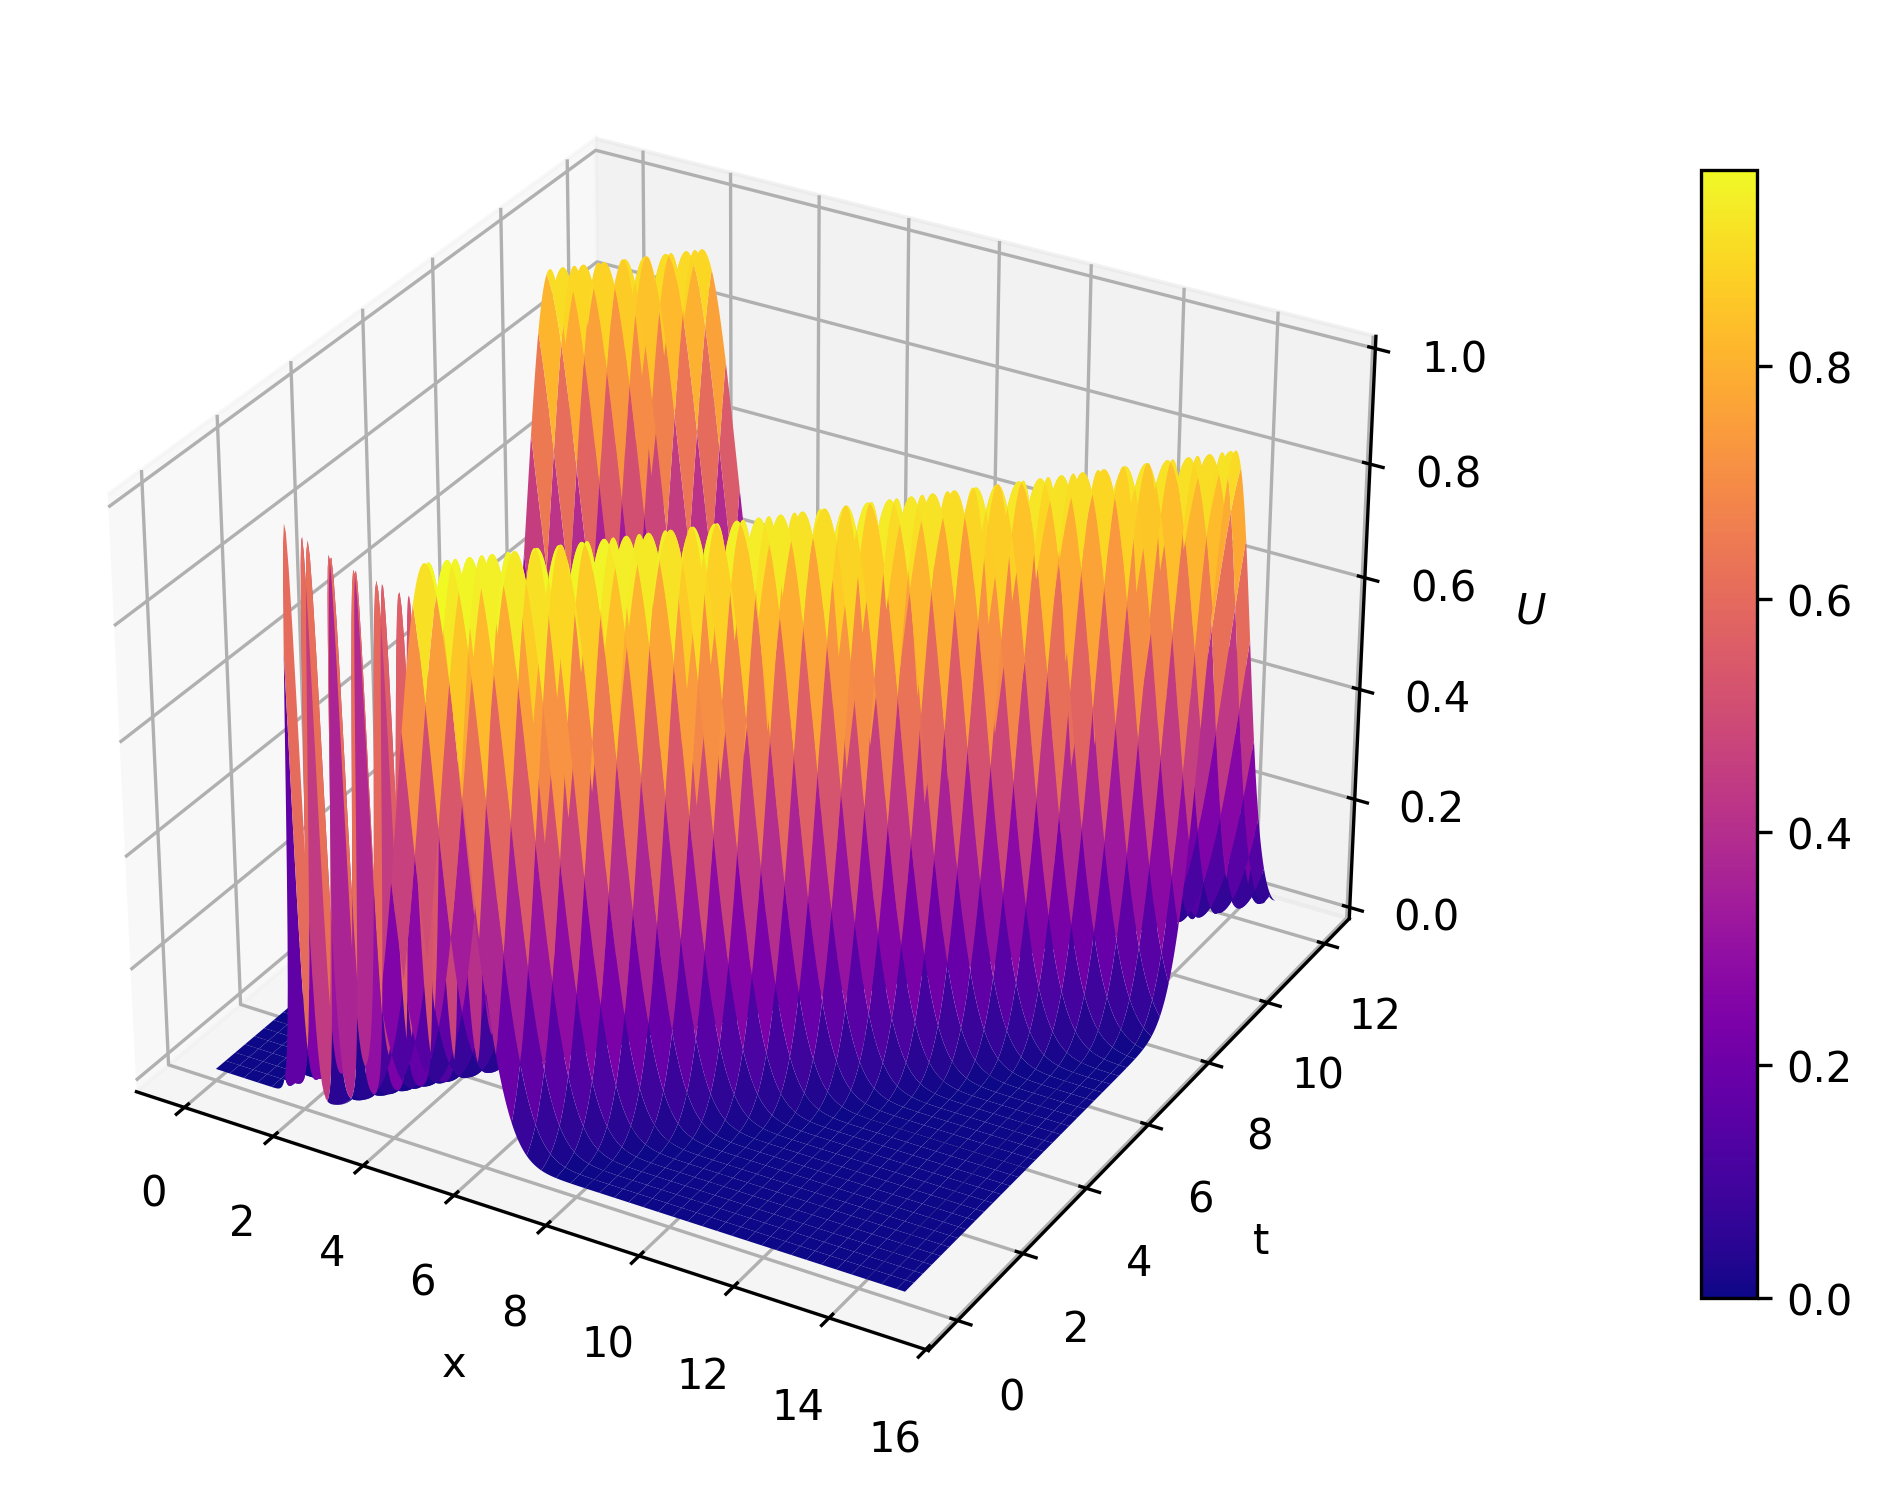
\includegraphics[width=\linewidth]{surface_upwind_Pe=1000.png}
            \caption{Solução com \textit{upwind} para $\bb{P}e = 1000$.}\label{fig:Pe1000up}
        \end{subfigure}

        \caption{Soluções numéricas com o esquema \textit{upwind} para valores crescentes de $\Pe$.}\label{fig:upwind}
    \end{figure}

    \newpage
    
    \subsection{Evolução Temporal da Solução}

    A influência dos efeitos advectivos e difusivos pode ser visualizada diretamente através de perfis de $u$ em função de $x$ para instantes de tempo distintos, conforme exibido nas Figuras~\ref{fig:timeupwind} e~\ref{fig:timecentral}.

    \begin{figure}[H]
        \centering

        \begin{subfigure}{0.45\textwidth}
            \centering
            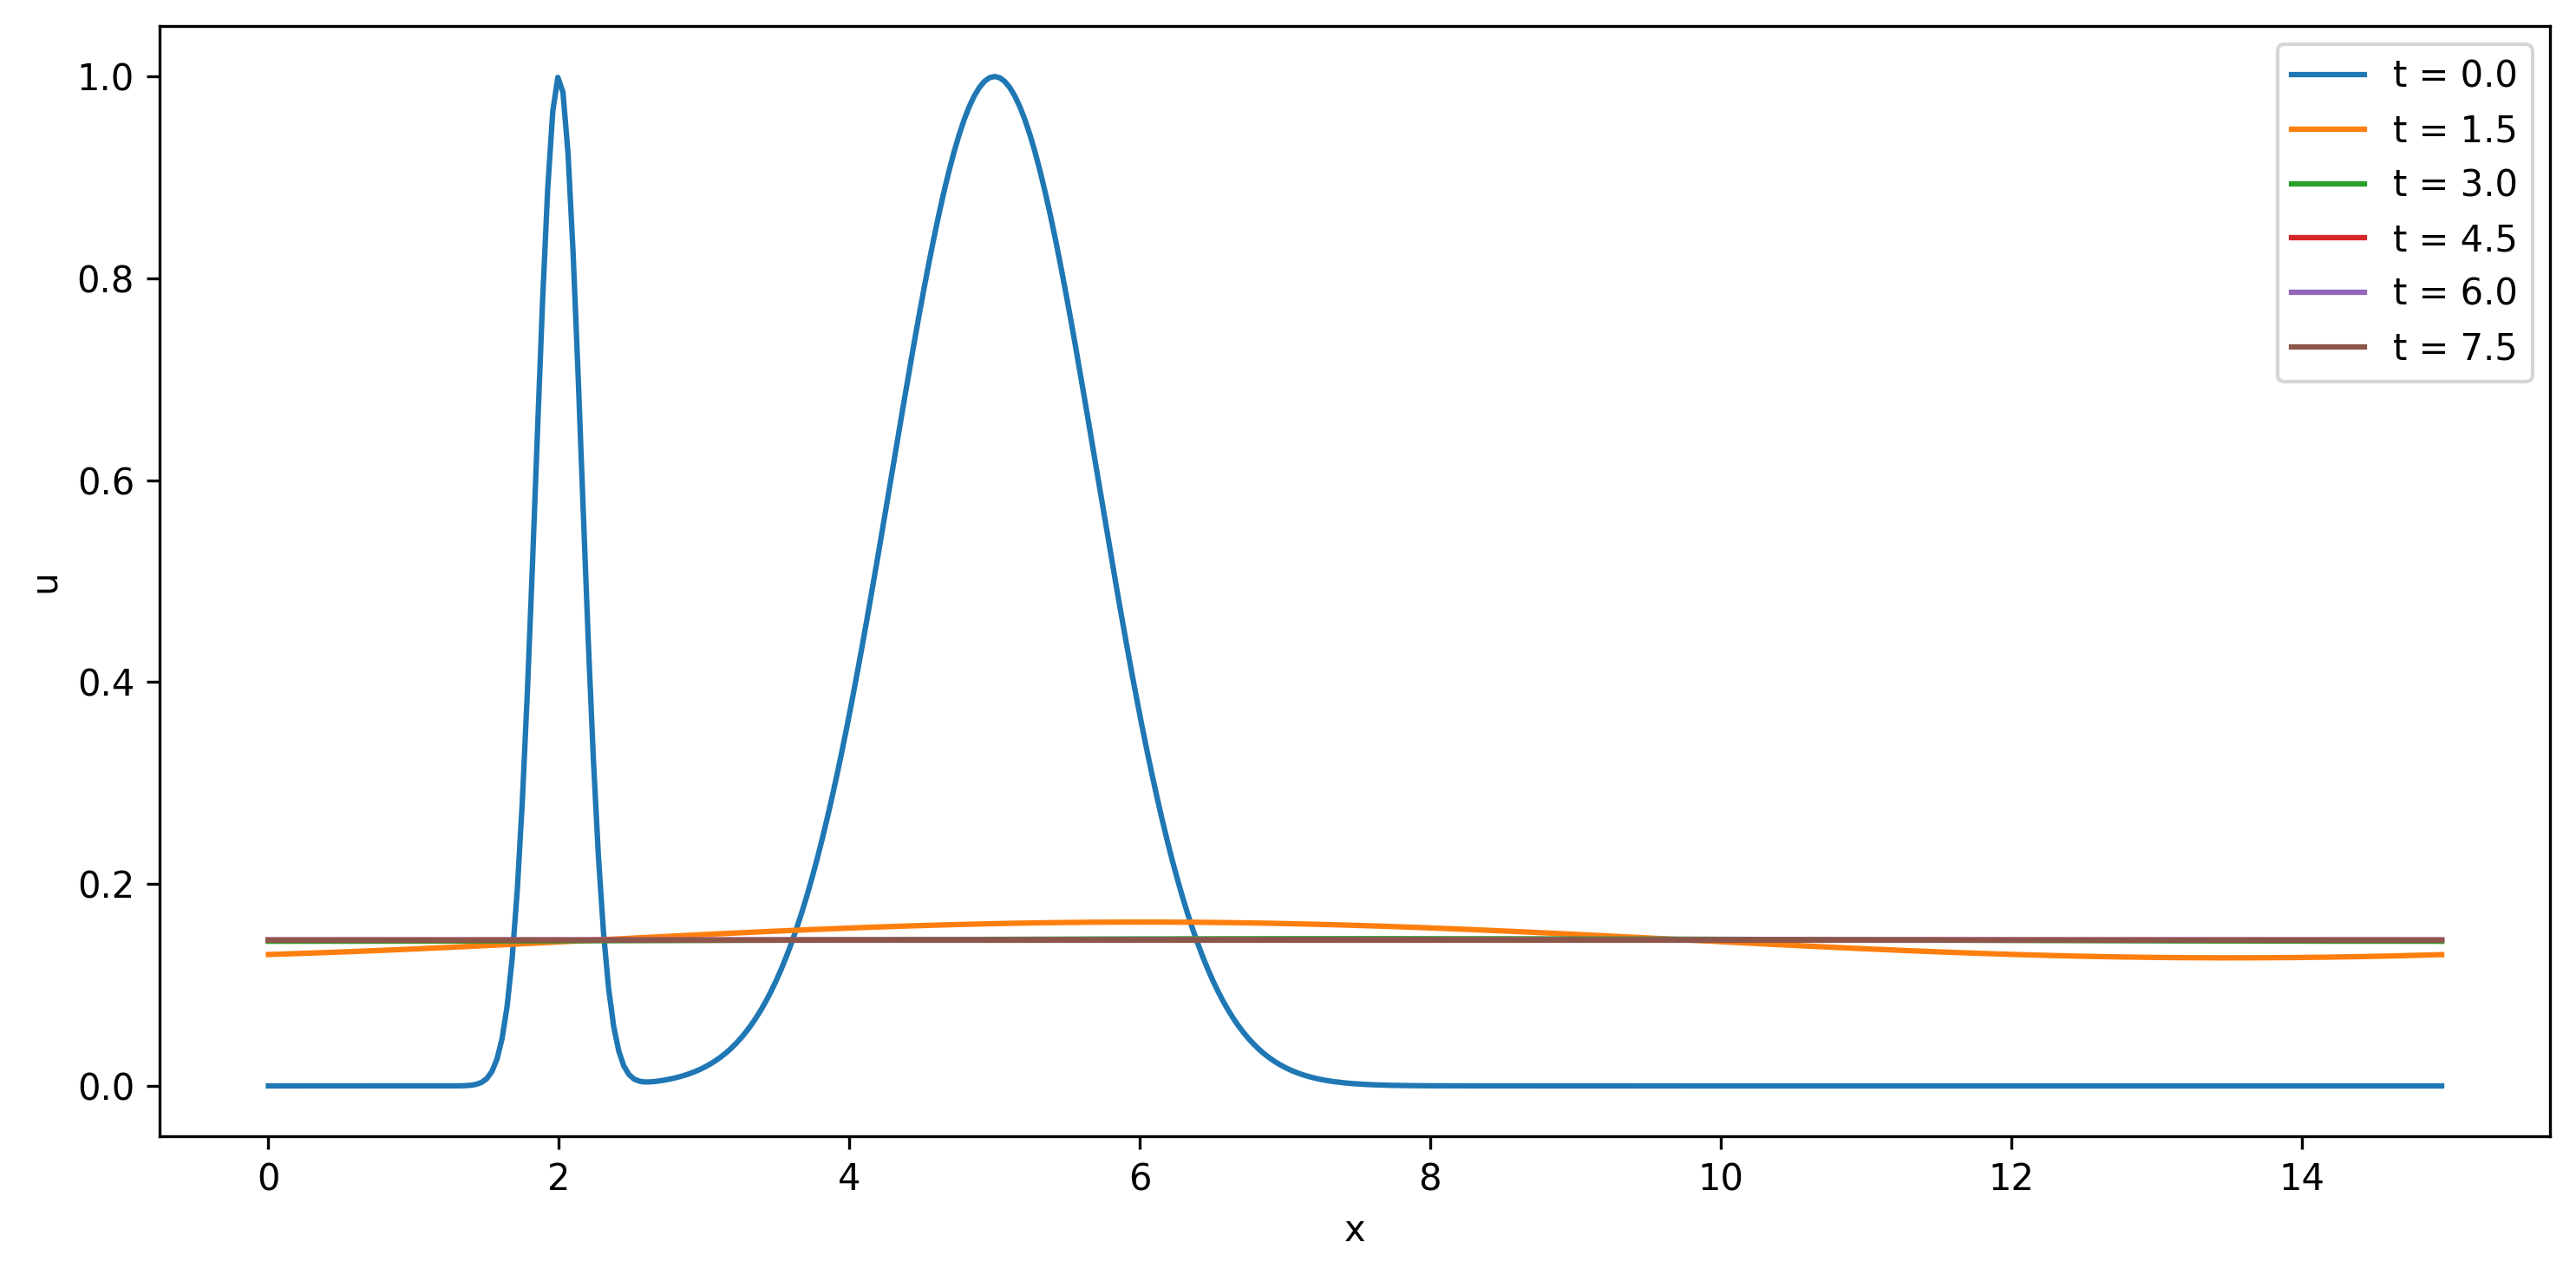
\includegraphics[width=\linewidth]{evol_upwind_Pe=0.1.png}
            \caption{\footnotesize Evolução temporal com \textit{upwind}, $\bb{P}e = 0{,}1$.}\label{fig:Pe01timeup}
        \end{subfigure}
        \hfill
        \begin{subfigure}{0.45\textwidth}
            \centering
            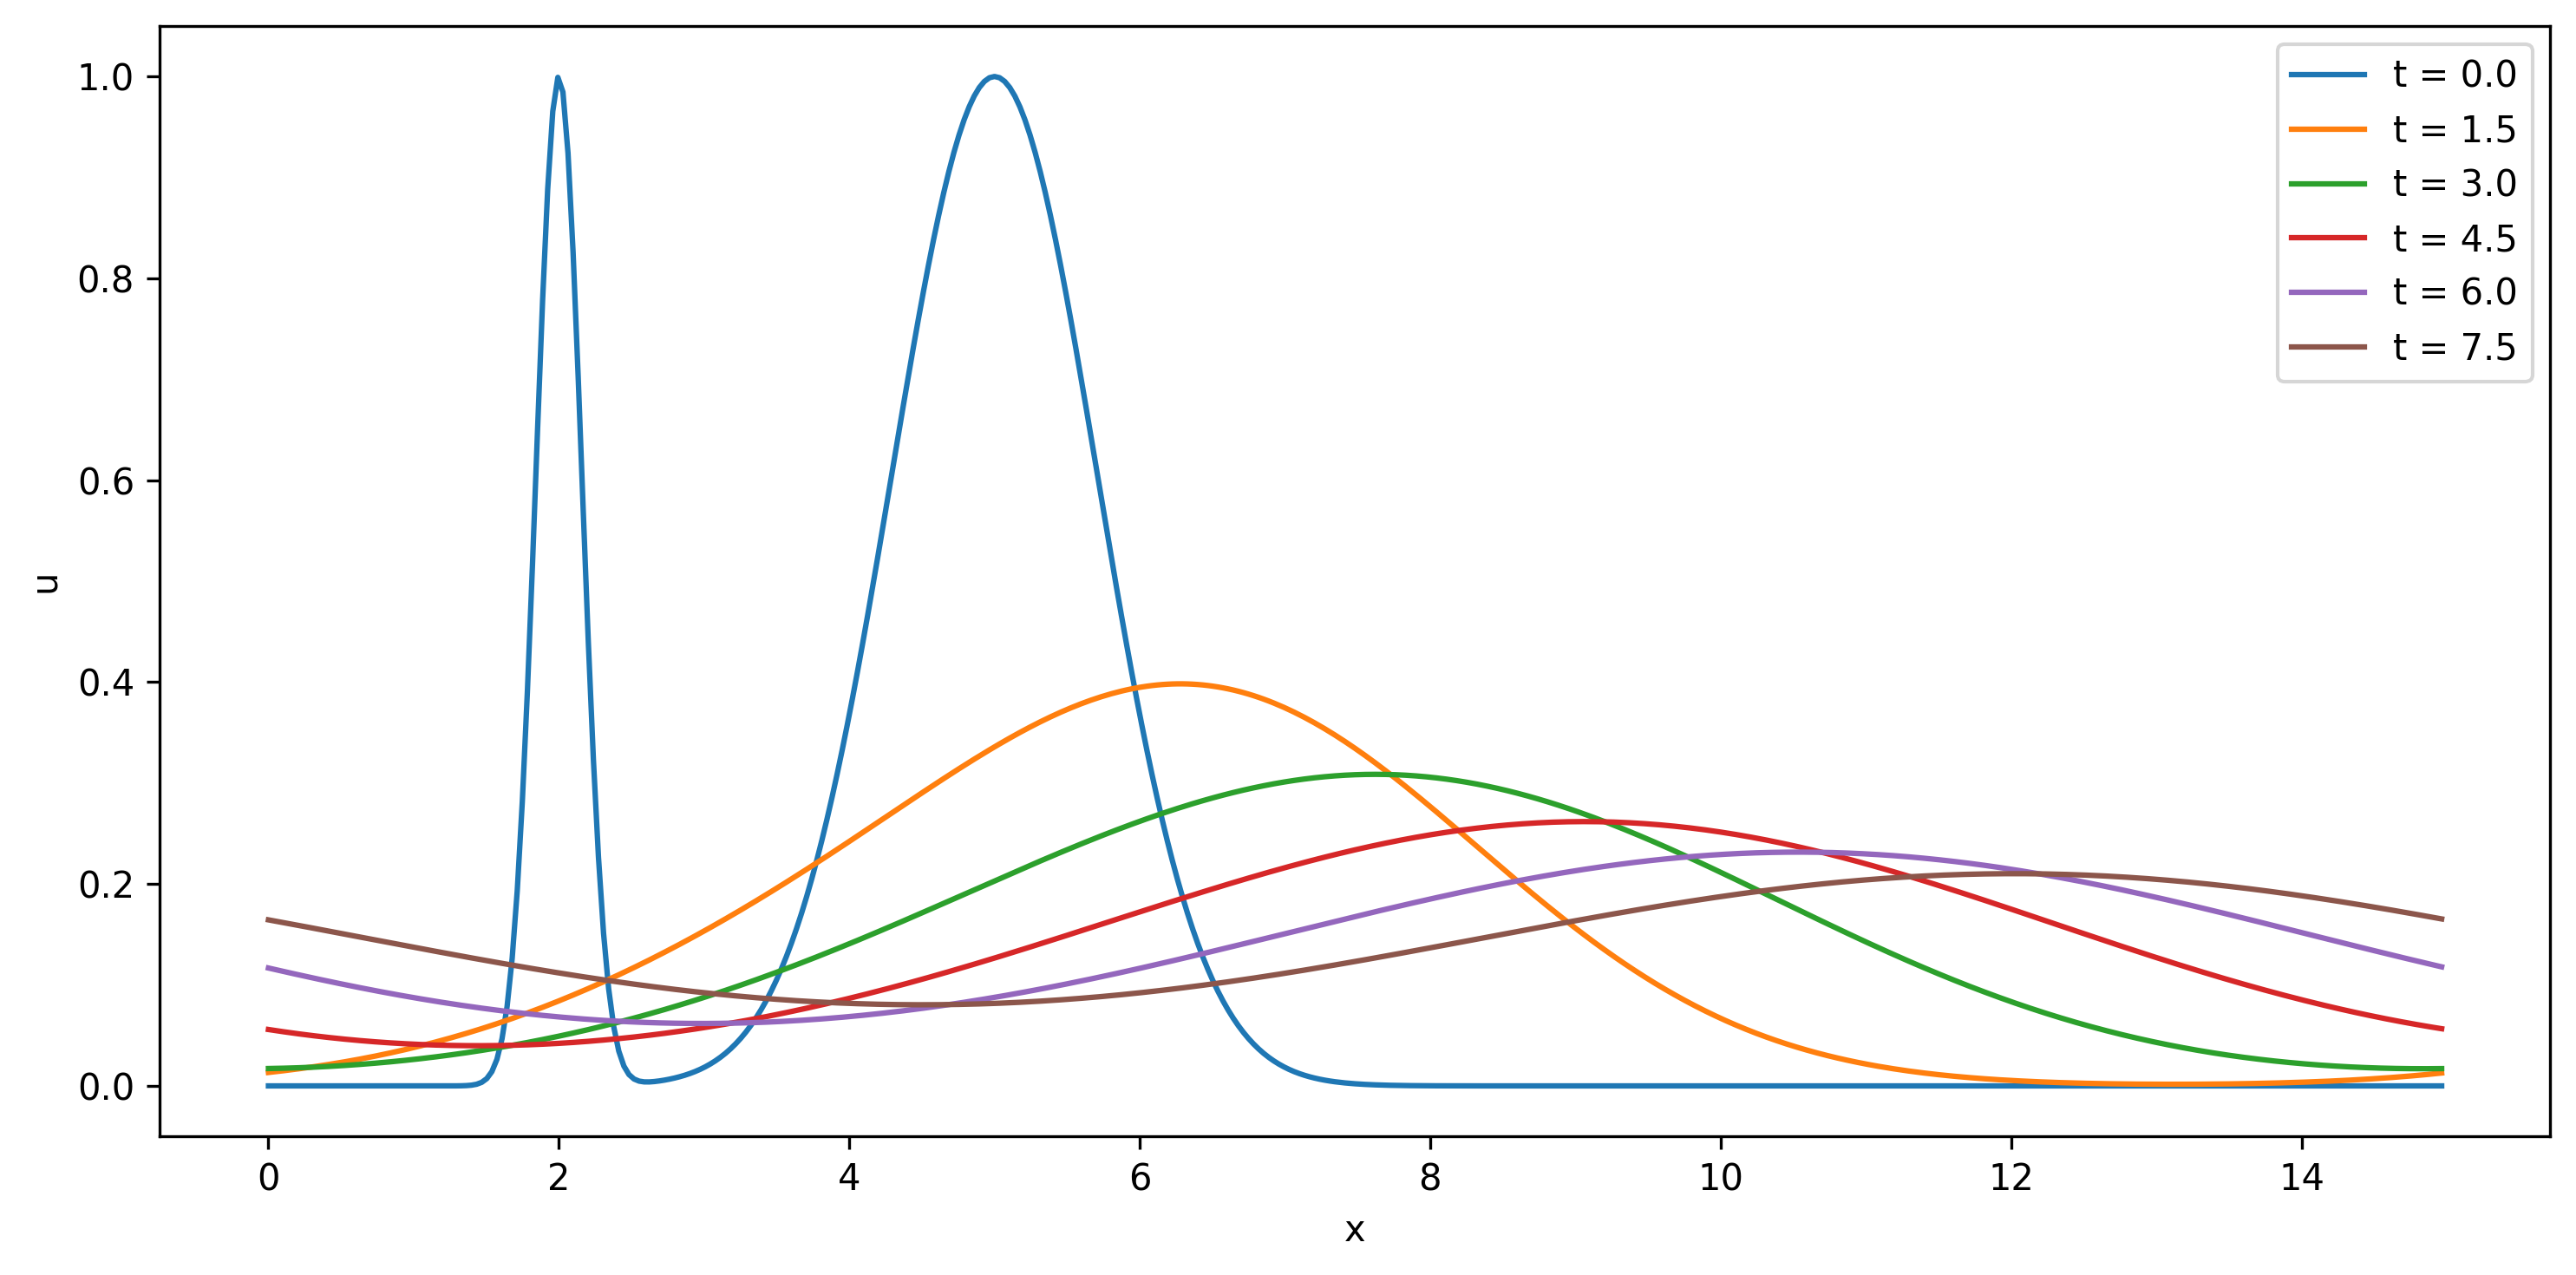
\includegraphics[width=\linewidth]{evol_upwind_Pe=1.png}
            \caption{\footnotesize Evolução temporal com \textit{upwind}, $\bb{P}e = 1$.}\label{fig:Pe1timeup}
        \end{subfigure}

        \vspace{0.5cm}

        \begin{subfigure}{0.45\textwidth}
            \centering
            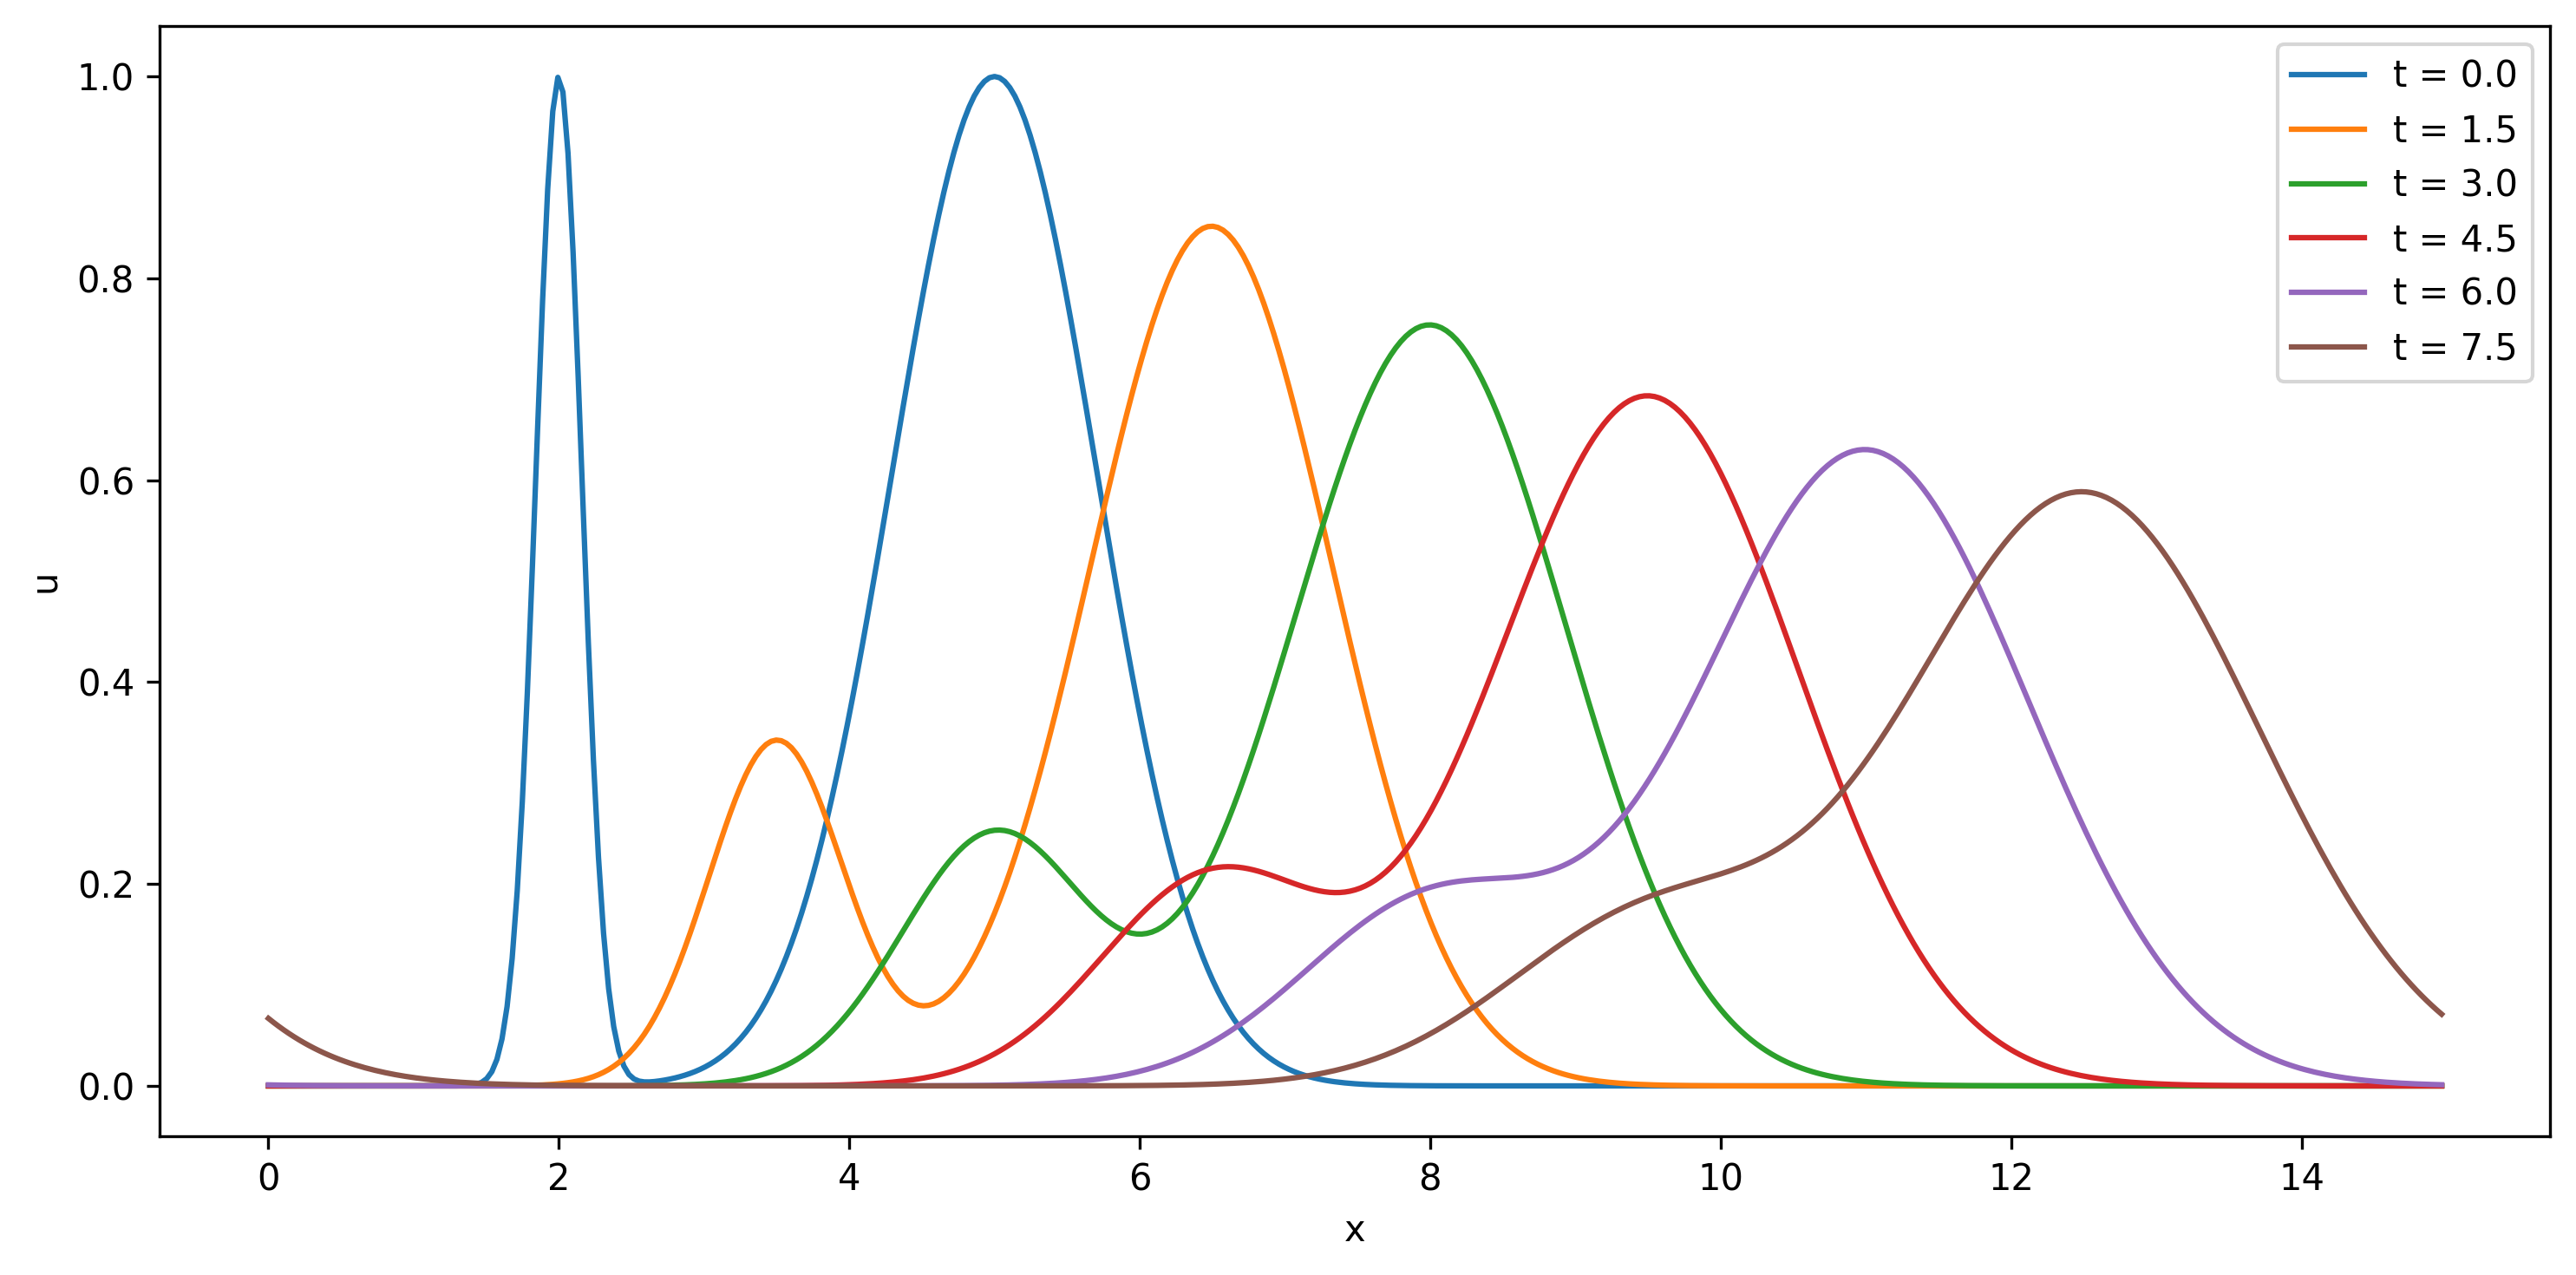
\includegraphics[width=\linewidth]{evol_upwind_Pe=20.png}
            \caption{\footnotesize Evolução temporal com \textit{upwind}, $\bb{P}e = 20$.}\label{fig:Pe20timeup}
        \end{subfigure}
        \hfill
        \begin{subfigure}{0.45\textwidth}
            \centering
            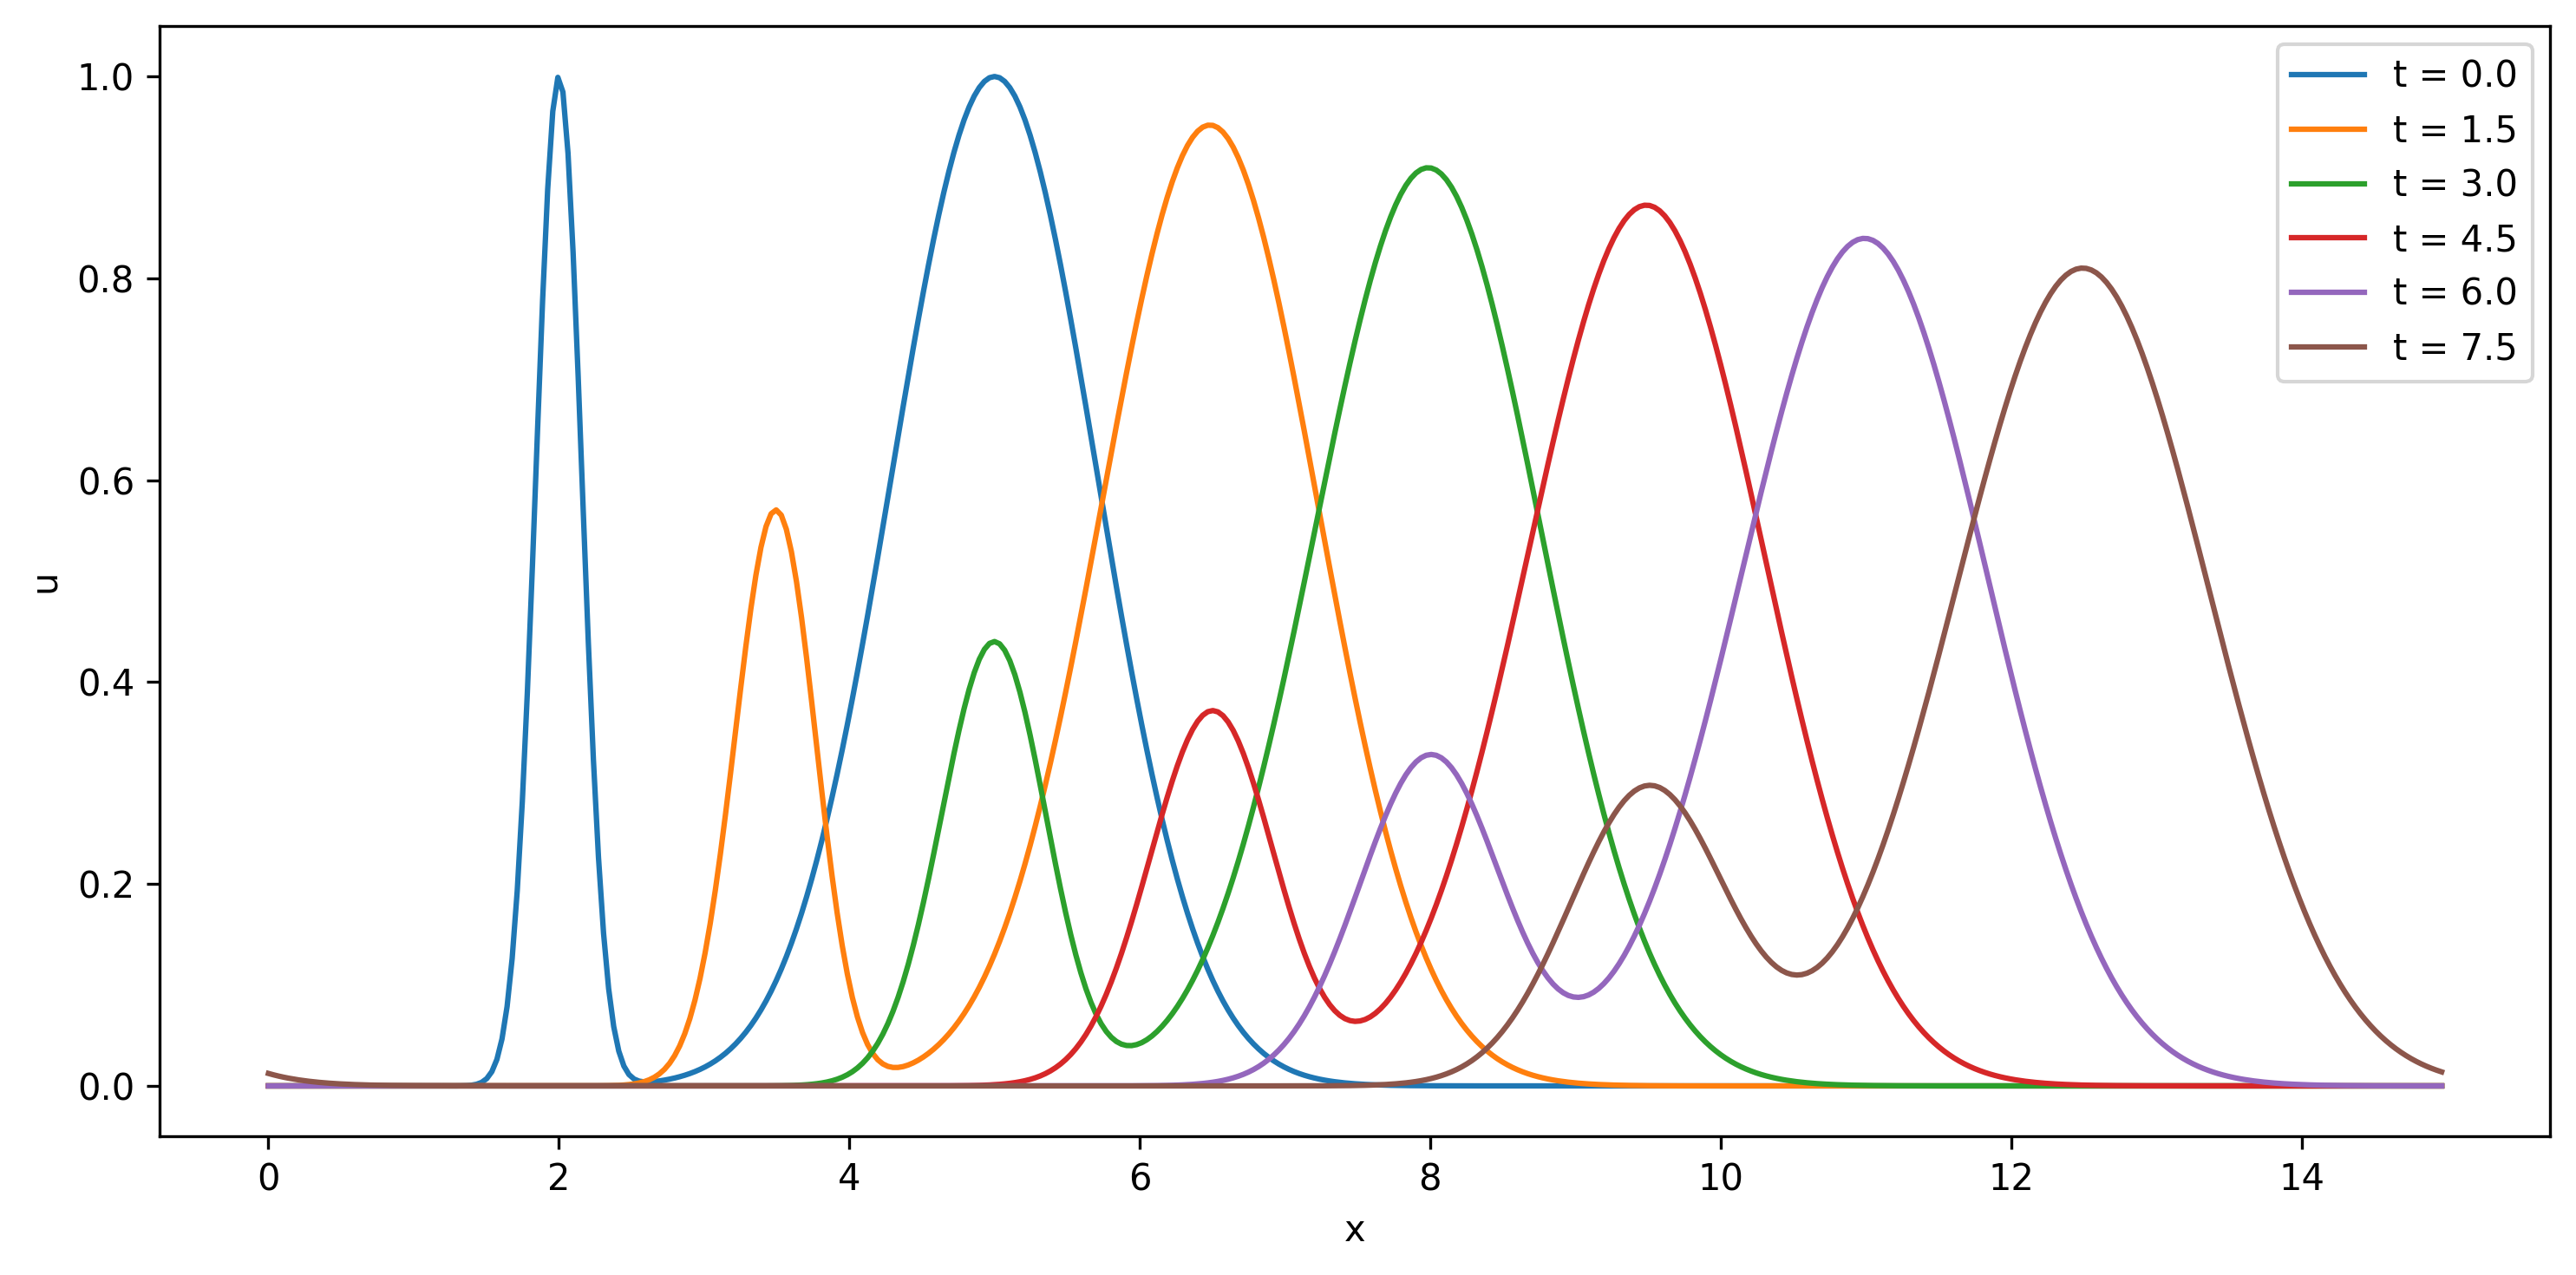
\includegraphics[width=\linewidth]{evol_upwind_Pe=100.png}
            \caption{\footnotesize Evolução temporal com \textit{upwind}, $\bb{P}e = 100$.}\label{fig:Pe100timeup}
        \end{subfigure}

        \caption{Efeito de distintos valores de $\Pe$ na solução obtida com o esquema \textit{upwind}.}\label{fig:timeupwind}
    \end{figure}

    \begin{figure}[H]
        \centering

        \begin{subfigure}{0.45\textwidth}
            \centering
            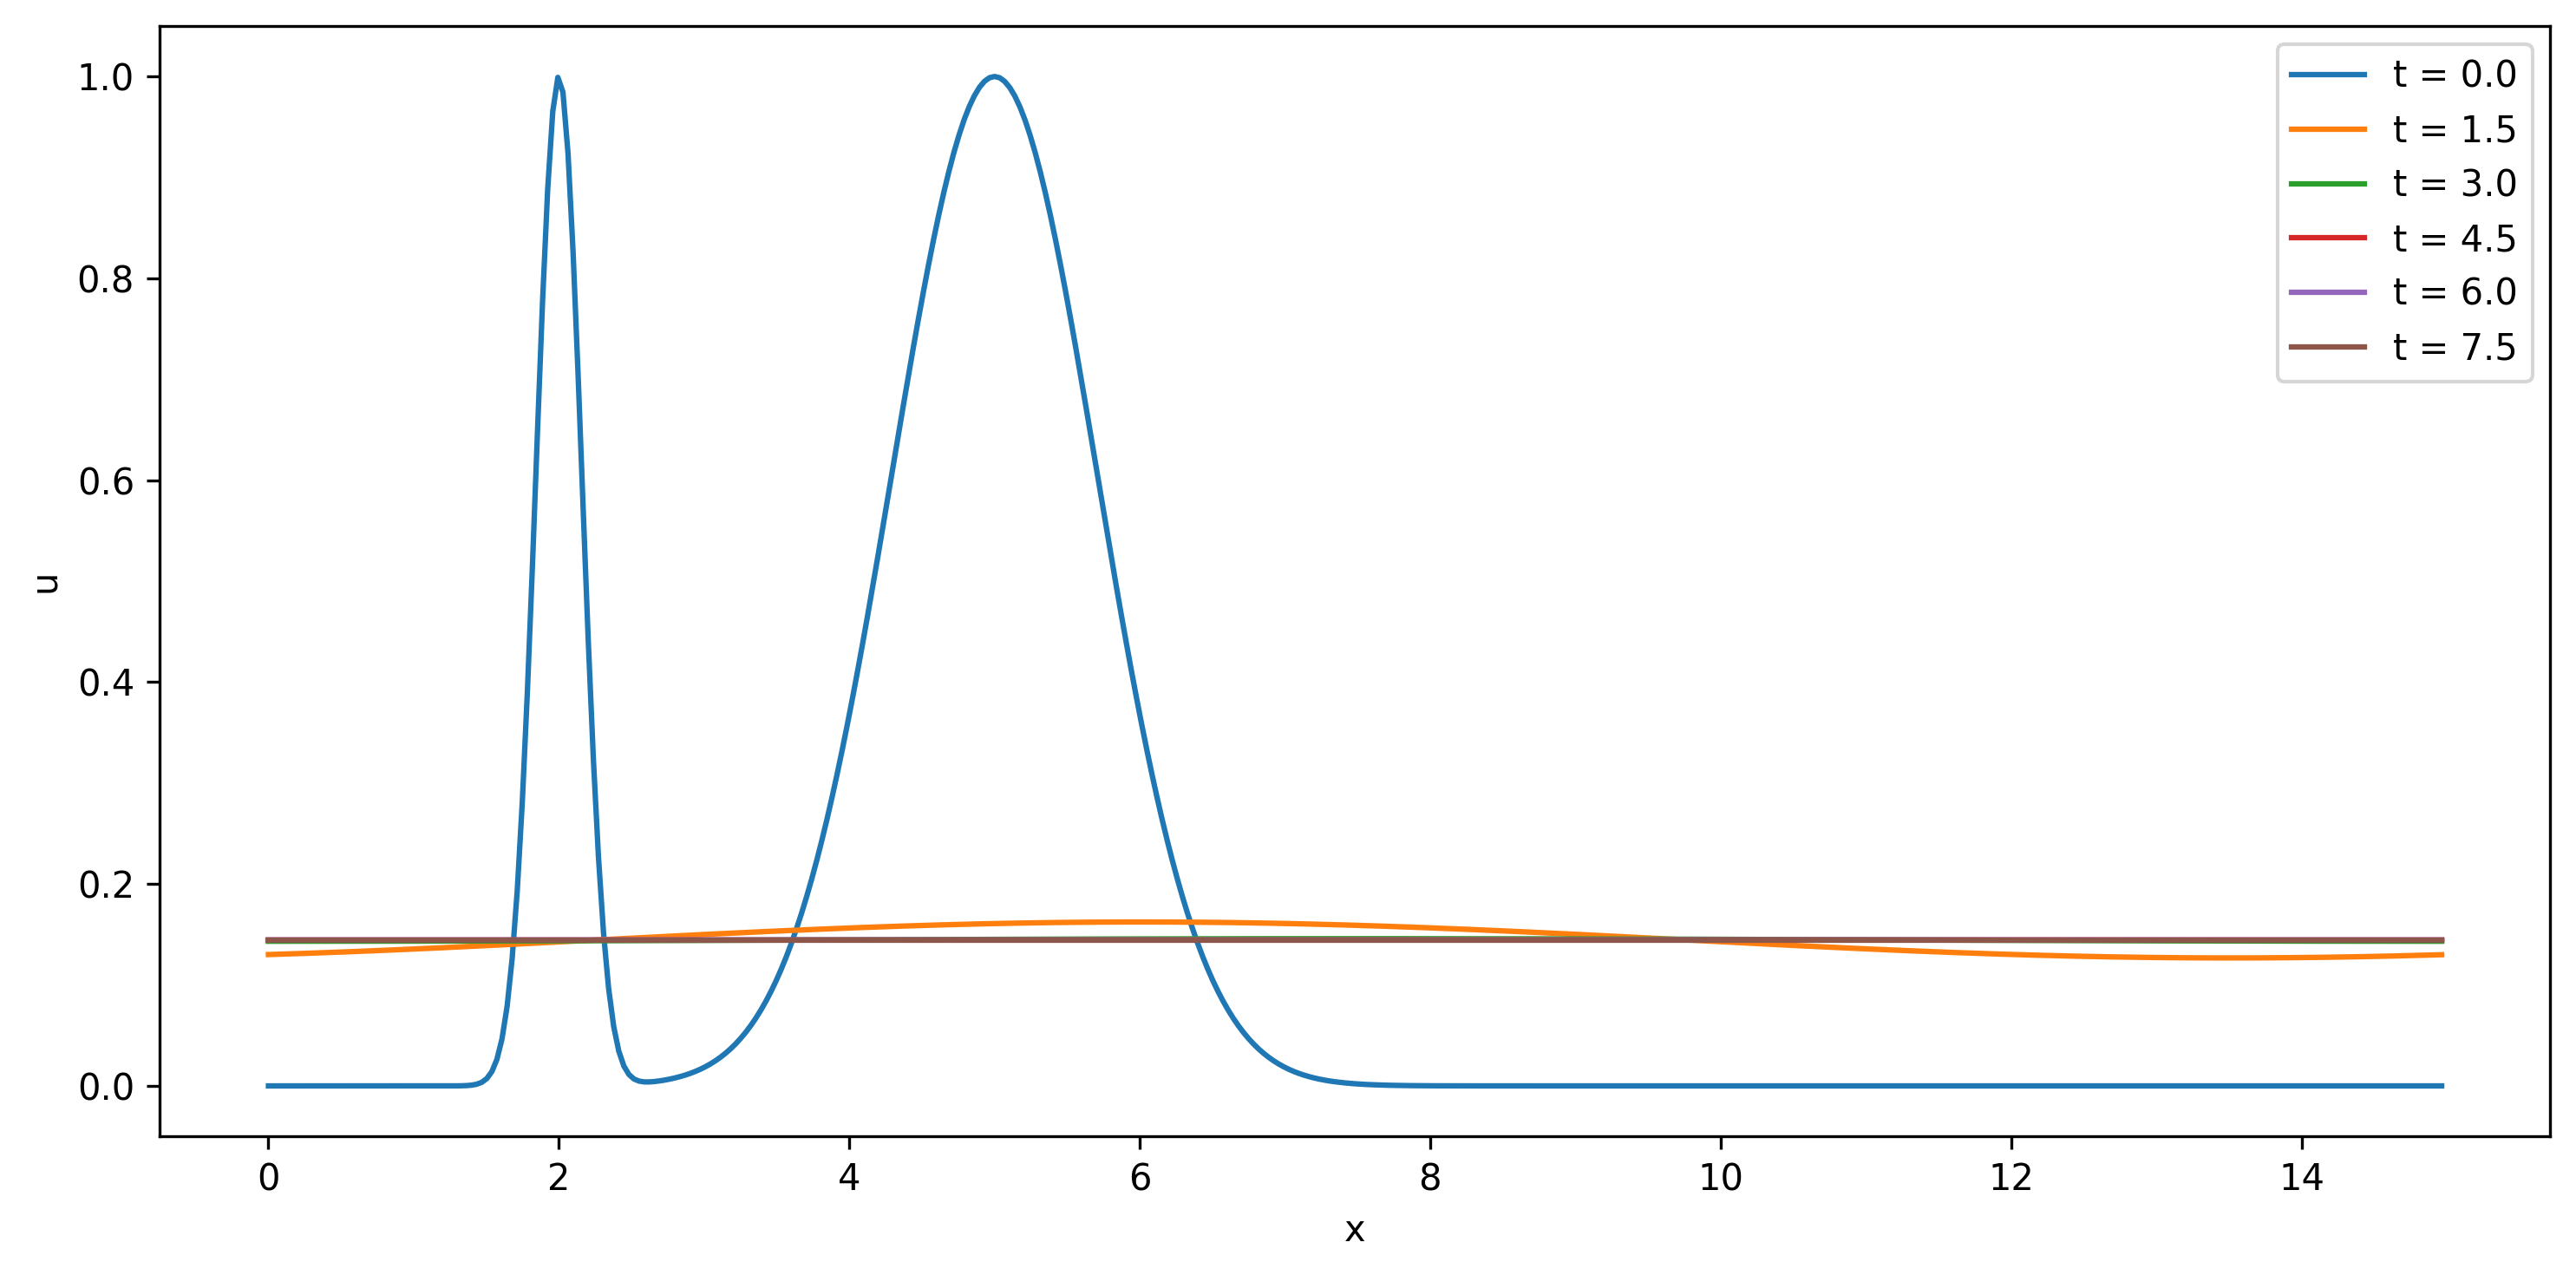
\includegraphics[width=\linewidth]{evol_central_Pe=0.1.png}
            \caption{Evolução temporal com discretização centrada, $\bb{P}e = 0{,}1$.}\label{fig:Pe01timecentral}
        \end{subfigure}
        \hfill
        \begin{subfigure}{0.45\textwidth}
            \centering
            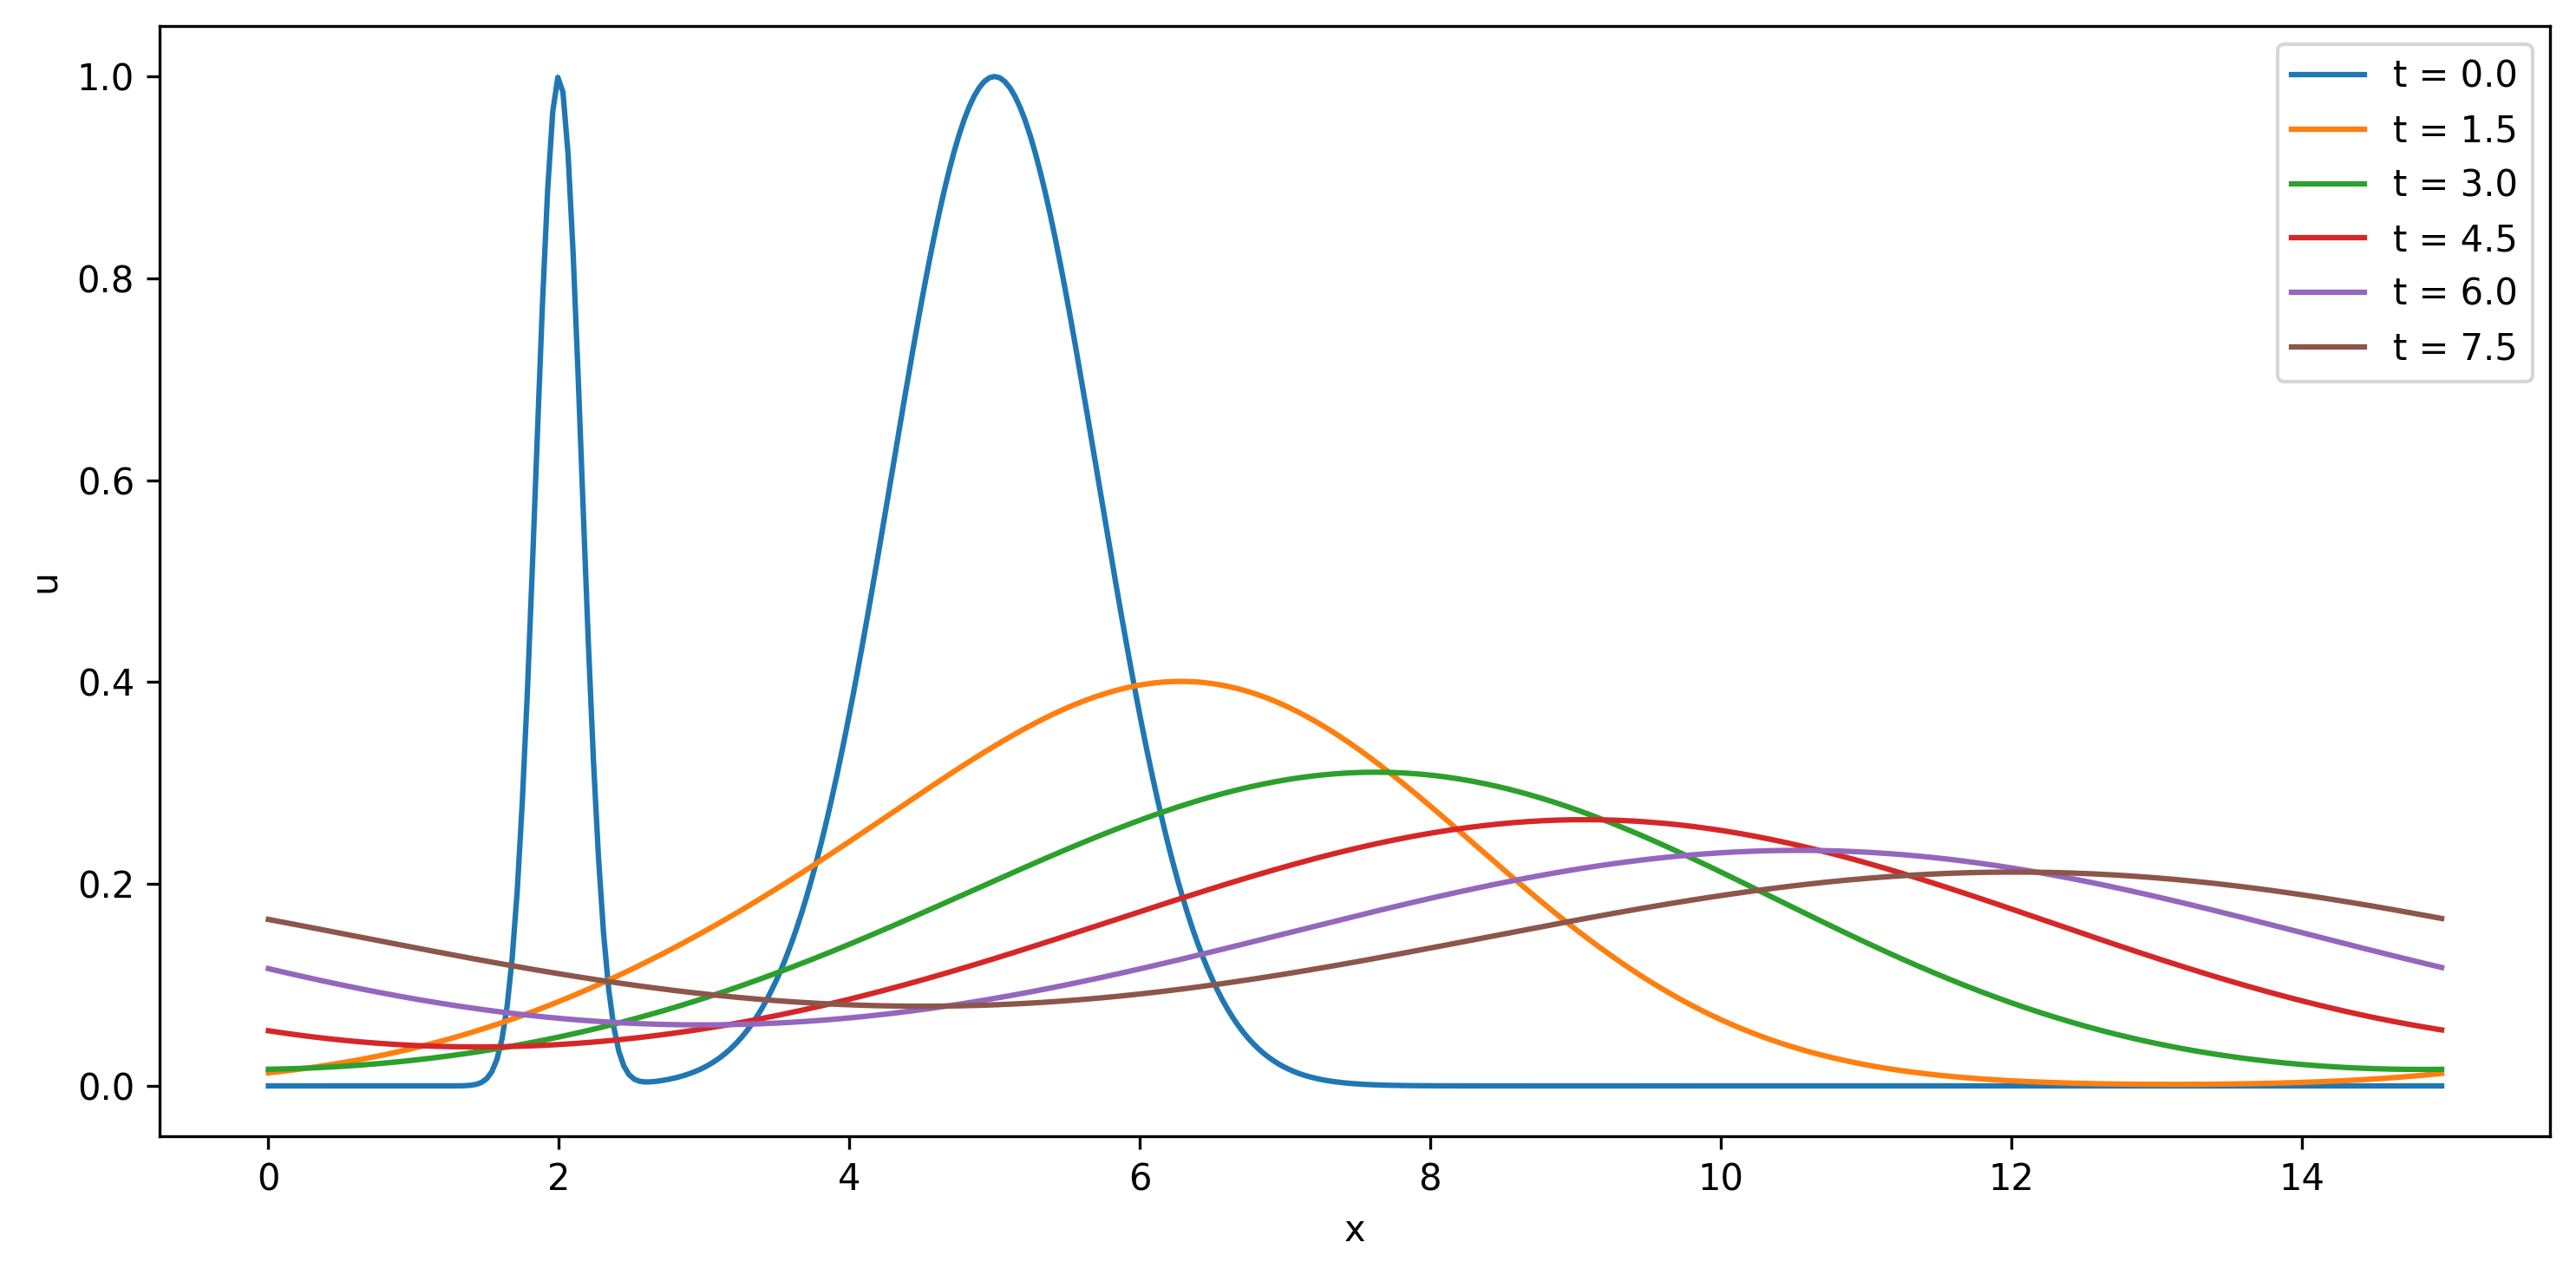
\includegraphics[width=\linewidth]{evol_central_Pe=1.png}
            \caption{Evolução temporal com discretização centrada, $\bb{P}e = 1$.}\label{fig:Pe1timecentral}
        \end{subfigure}

        \vspace{0.5cm}

        \begin{subfigure}{0.45\textwidth}
            \centering
            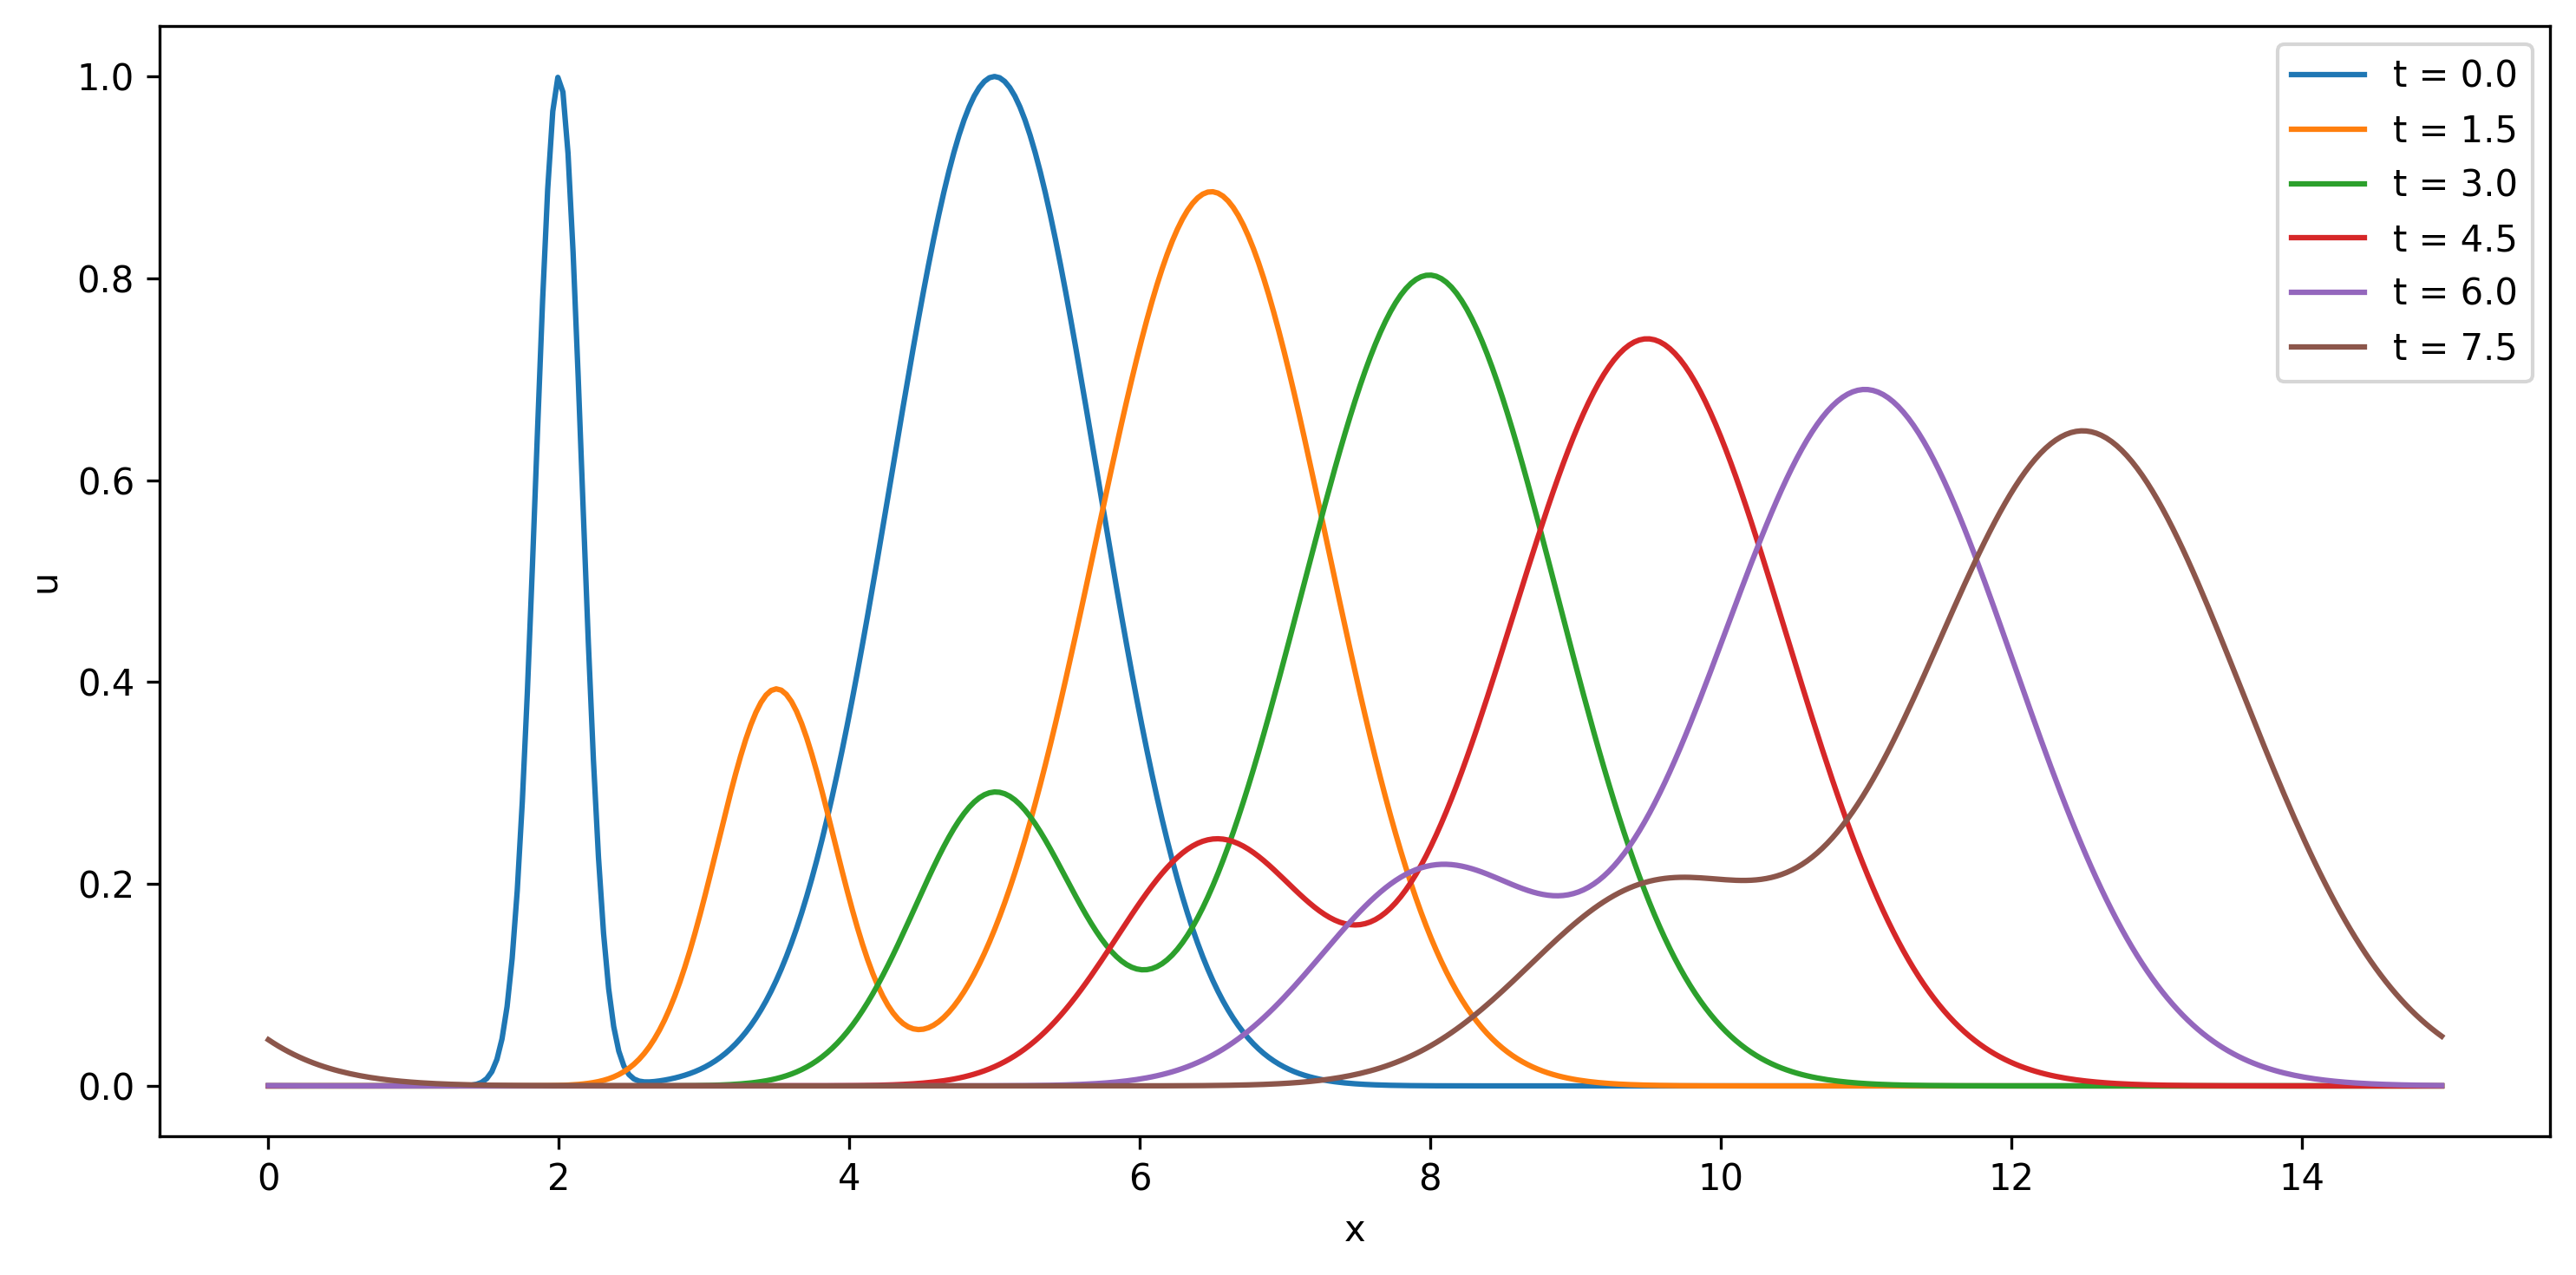
\includegraphics[width=\linewidth]{evol_central_Pe=20.png}
            \caption{Evolução temporal com discretização centrada, $\bb{P}e = 20$.}\label{fig:Pe20timecentral}
        \end{subfigure}
        \hfill
        \begin{subfigure}{0.45\textwidth}
            \centering
            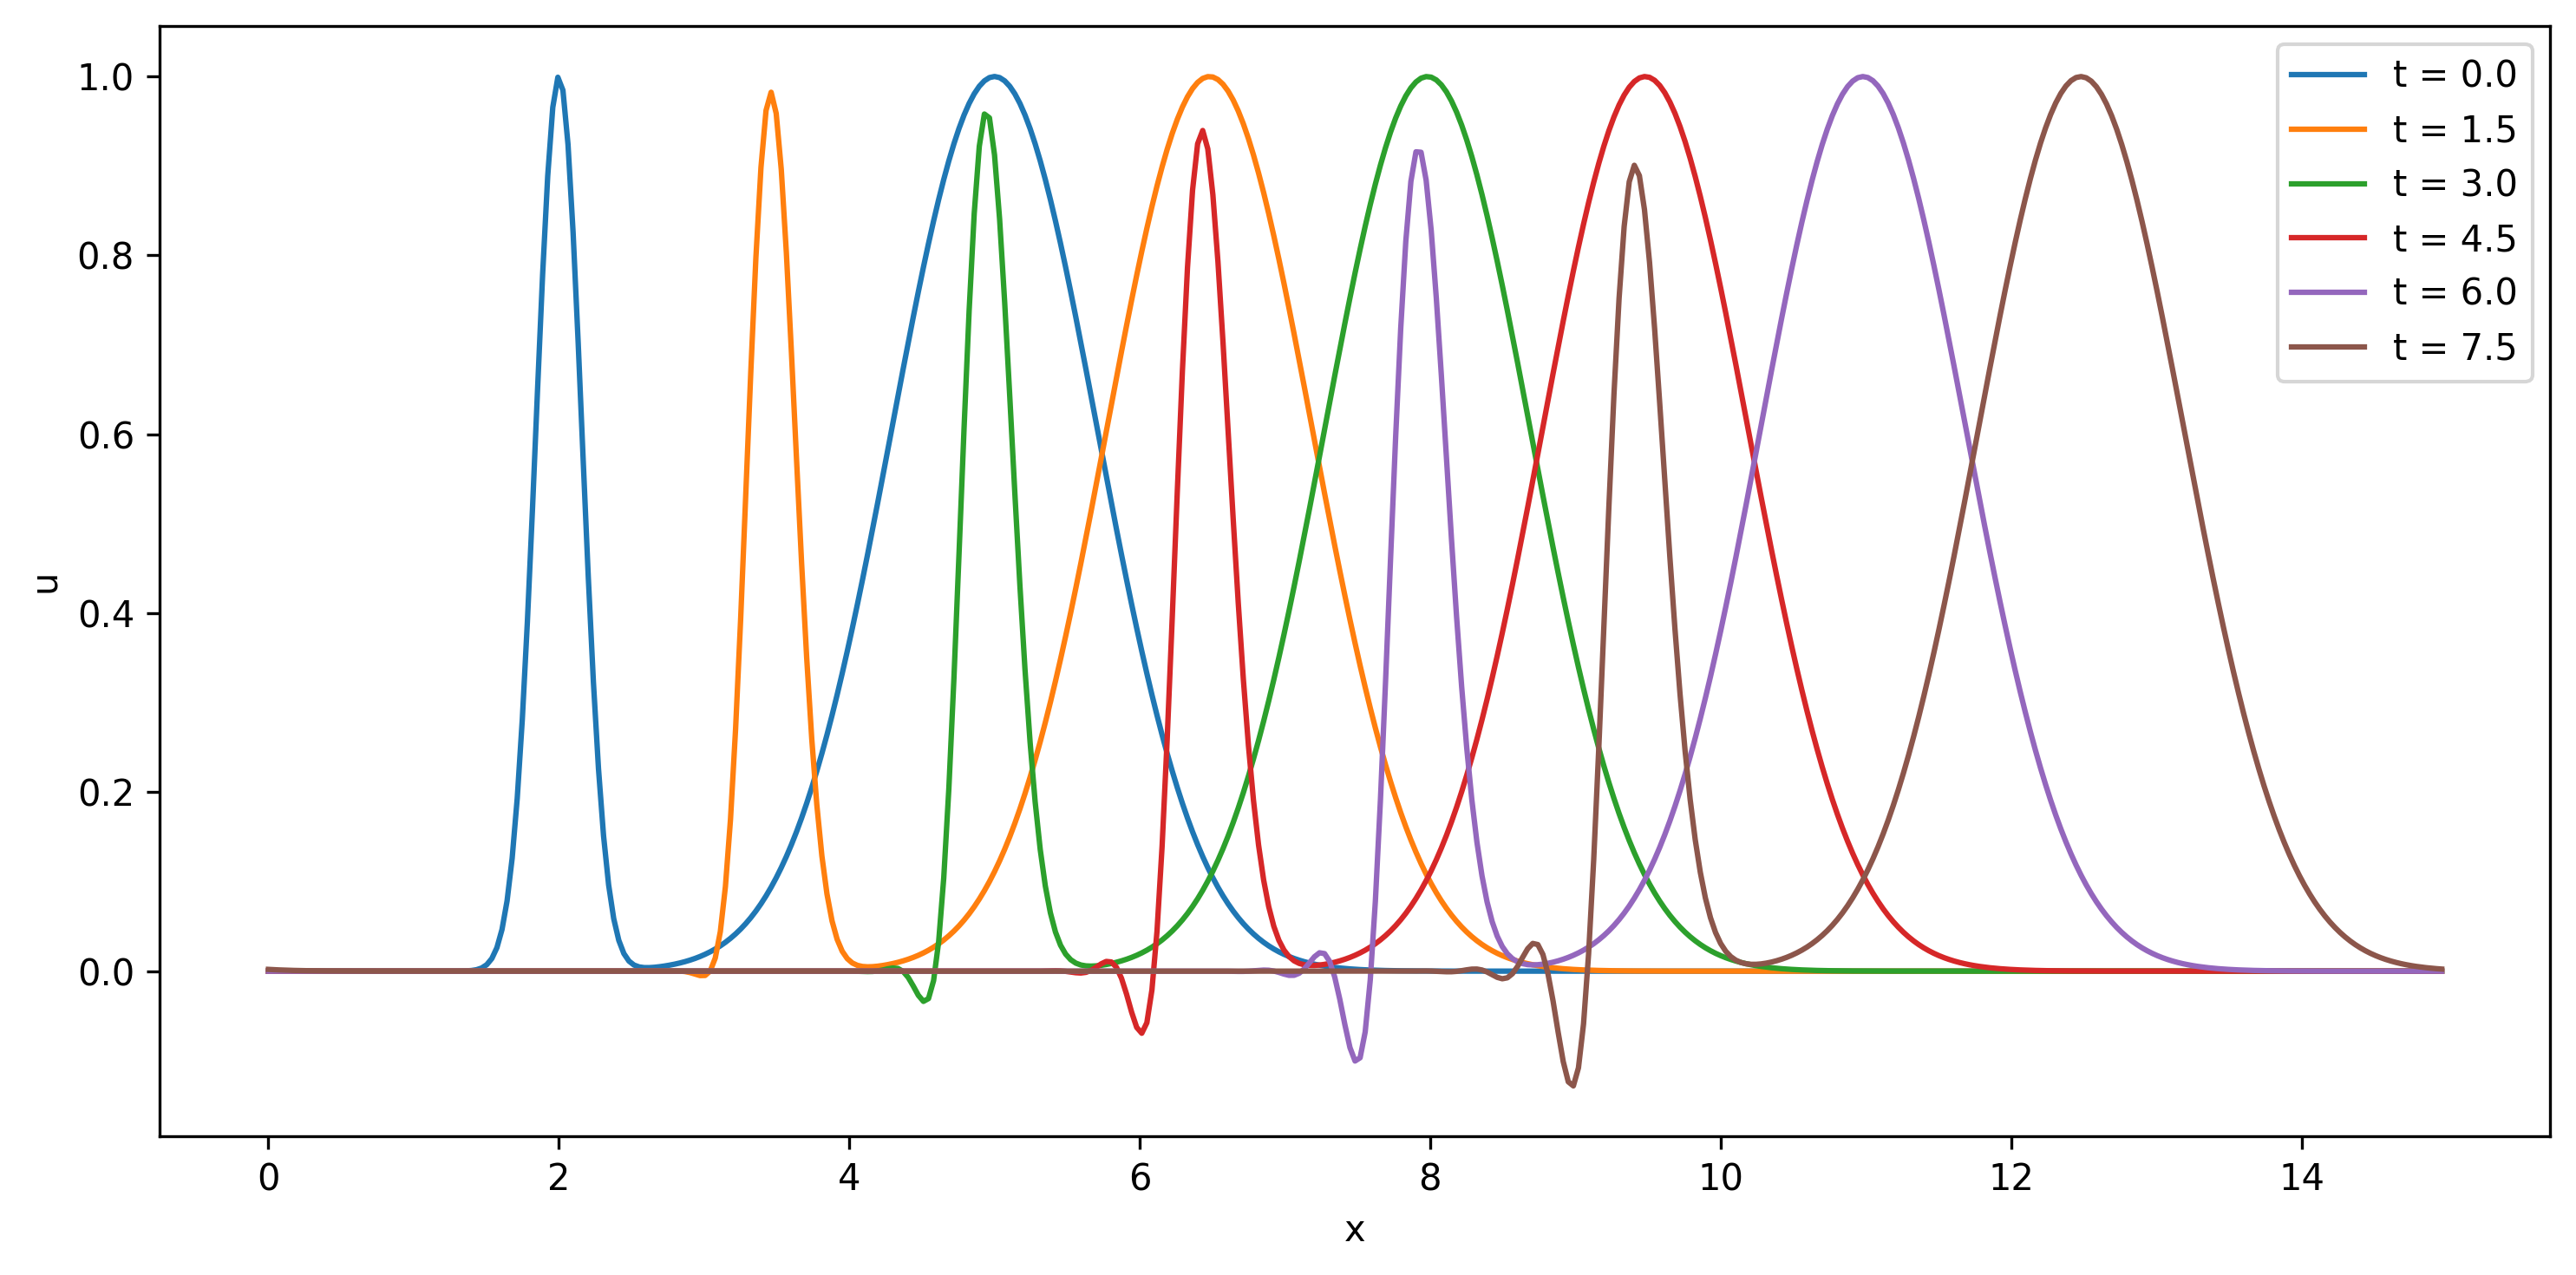
\includegraphics[width=\linewidth]{evol_central_Pe=100.png}
            \caption{Evolução temporal com discretização centrada, $\bb{P}e = 100$.}\label{fig:Pe100timecentral}
        \end{subfigure}

        \caption{Efeito de distintos valores de $\Pe$ na solução obtida com o esquema de diferenças centradas.}\label{fig:timecentral}
    \end{figure}

    Para $\Pe \ll 1$, a difusividade supera a advecção em escala, e a solução converge rapidamente para um perfil aproximadamente uniforme. Para $\Pe = 1$, advecção e difusão atuam em proporções comparáveis. No regime $\Pe \gg 1$, a advecção passa a dominar e os pulsos iniciais são transportados com atenuação mínima. Nesse limite, a discretização centrada preserva melhor a baixa difusividade, ao passo que o esquema \textit{upwind} introduz difusão numérica artificial; contudo, o esquema centrado exibe oscilações espúrias nas proximidades dos picos de maior gradiente.

    \section{Análise das Restrições de Estabilidade}

    Conforme estabelecido na Seção~\ref{sec:peclet}, a condição $\D{t} < R_1 \equiv \dfrac{\D{x^2}}{\frac{2}{\Pe} + \D{x}}$ é sempre mais restritiva do que a condição CFL $\D{t} < R_2 \equiv \D{x}$. Os comportamentos assintóticos de $R_1$ são:

    Para $\Pe \to \infty$:
    \[
        R_1 \to \D{x},
    \]

    para $\Pe \to 0^+$:
    \[
        R_1 \to \frac{\Pe \D{x^2}}{2}.
    \]

    Essa dependência é ilustrada na Figura~\ref{fig:loglog}.

    \begin{figure}[H]
        \centering
        \begin{subfigure}{0.45\textwidth}
            \centering
            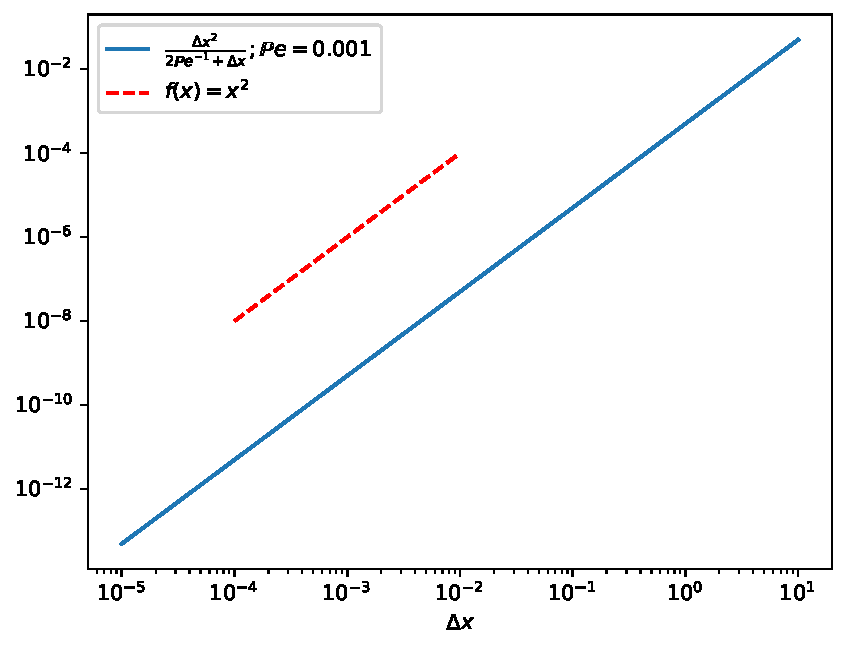
\includegraphics[width=\linewidth]{retricao_Pe=0.001.pdf}
            \caption{$R_1$ em função de $\D{x}$ para $\bb{P}e = 0{,}001$.}\label{fig:restricao_pe}
        \end{subfigure}
        \hfill
        \begin{subfigure}{0.45\textwidth}
            \centering
            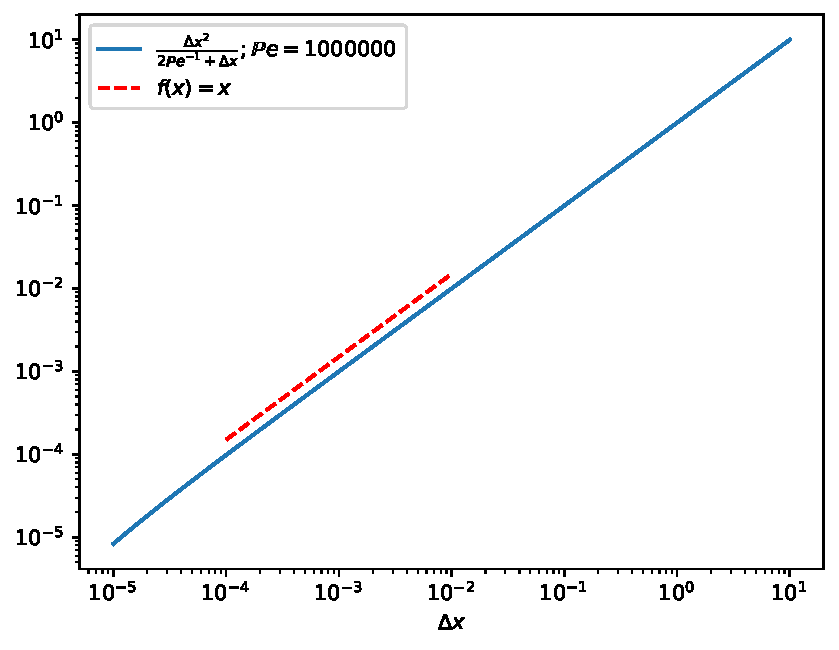
\includegraphics[width=\linewidth]{retricao_Pe=1000000.pdf}
            \caption{$R_1$ em função de $\D{x}$ para $\bb{P}e = 10^6$.}\label{fig:restricao_PE}
        \end{subfigure}
        \caption{Comportamento assintótico da restrição de estabilidade $R_1$ nos regimes de $\Pe$ pequeno e grande.}\label{fig:loglog}
    \end{figure}

    Quando $\Pe$ é pequeno, a restrição sobre $\D{t}$ apresenta dependência quadrática em $\D{x}$, tornando-se significativamente mais severa e aumentando o custo computacional dos esquemas explícitos. Nesse regime, métodos implícitos, que são incondicionalmente estáveis, tornam-se alternativas mais atrativas. Para $\Pe$ elevado, a restrição temporal é menos severa; porém, como discutido, o esquema centrado pode exibir instabilidade numérica nesse limite.

\end{document}